
\begin{apendicesenv}

\partapendices

\chapter{Aposentadoria no Brasil}

Aposentar-se é o ato de afastar-se de atividades profissionais. Após um período de contribuição em algum plano de aposentadoria, seja ele público ou privado, pode se ter um afastamento remunerado por tempo indeterminado. No Brasil, a aposentadoria é um direito garantido pela Constituição Federativa do Brasil (CF), no artigo 201 (BRASIL,1988). Tem-se para tanto um Ministério responsável por amparar o trabalhador quanto aos seus direitos. Existe hoje no Brasil três Regimes Previdenciários: (i) o regime próprio (BRASIL, Constituição,1988, artigo 40), este para servidores públicos, no qual o órgão em que ele está lotado possui um regime previdenciário; (ii) o regime geral (BRASIL, Constituição,1988, artigo 201), este de natureza obrigatória e vínculo automático ao trabalhador de empresas privadas e públicas, sempre quando essas não possuírem um regime previdenciário próprio; (iii) e o regime complementar (BRASIL, Constituição,1988,artigo 202) (BRASIL, Emenda Constitucional nº 20,1998), este de caráter facultativo. Pode ser do tipo fechado (BRASIL, Lei Complementar 108, 2001), ou seja, somente para trabalhadores que possuem vínculos empregatícios em uma determinada empresa. Mas, também pode ser do tipo aberto (BRASIL, Lei Complementar 109, 2001), ou seja, não vinculado ao trabalho, e normalmente gerido por empresas financeiras.

O regime geral de previdência é administrado pelo Instituto Nacional do Seguro Nacional, INSS. Trata-se de um Órgão vinculado ao Ministério da Previdência Social, criado em 24 de junho de 1990 (BRASIL, Decreto nº 99.350, 1990). Entretanto, o direito previdenciário existe desde 24 de janeiro de 1923, com o Decreto 4.682/23 (BRASIL, 1923). Os decretos supracitados garantem o direito à previdência ao trabalhador, denominado assegurado, e seus dependentes. São reconhecidos como dependentes (BRASIL,Lei nº 8.213, 1991, Art. 16): (i) o cônjuge, a companheira, o companheiro e o filho não emancipado, de qualquer condição, menor de 21 anos ou inválido ou que tenha deficiência intelectual que o torne absoluta ou relativamente incapaz, assim declarado judicialmente; (ii) os pais; (iii) e o irmão não emancipado, de qualquer condição, menor de 21 anos ou que tenha deficiência intelectual. No caso destes últimos, o INSS dispõe de pensão por morte e auxilio reclusão, quando o assegurado vinculado morre ou mesmo cumpre pena em regime carcerário.

Vale ressaltar ainda que todas as pessoas físicas brasileiras são asseguradas, as quais são divididas em segurados obrigatórios e facultativos (BRASIL, Lei nº 8.213, 1991 Art. 11). São denominados segurados obrigatórios: (i) todos os trabalhadores que prestam serviços de natureza urbana ou rural à empresa, em caráter não eventual, sob sua subordinação e mediante remuneração, inclusive como diretor empregado; (ii) empregados domésticos, aqueles que prestam serviços de natureza contínua a uma pessoa ou família, no âmbito residencial desta, em atividades sem fins lucrativos; (iii) contribuinte individual, que são fazendeiros, pescadores e garimpeiros; (iv) trabalhadores avulsos, aqueles que prestam serviços para diversas empresas, sem vínculo empregatício, serviço de natureza urbana ou rural. São denominados segurados facultativos, todos os indivíduos maiores de 14 anos que se afiliam ao regime geral de previdência social, mediante contribuição, desde que não incluído nas disposições do artigo 11 (BRASIL, Lei nº8.213, 1991, Art. 13).

Os segurados obrigatórios são vinculados de maneira automática ao INSS. Para estes são oferecidos oito benefícios (BRASIL, Lei nº 8.213,1991, Art. 18), expostos abaixo:

\begin{itemize}
\item Aposentadorias

		\begin{itemize}
		\item Aposentadoria por idade: 65 para homens e 60 para mulheres;
		\item Aposentadoria por tempo de contribuição: 35 para homes e 30 mulheres;
		\item Aposentadoria por invalidez: em virtude de acidentes que invalide o segurado, de maneira permanente, à executar atividades profissionais;
		\item Aposentadoria especial: para profissionais que lidam com agentes químicos ou biológicos, os quais são considerados nocivos à sua saúde;

		\end{itemize}
\item Auxílios

		\begin{itemize}
		\item Auxílio doença: em períodos de doença, a qual impeça o segurado na realização de atividades profissionais de maneira temporária;
		\item Auxilio acidente: para acidentes ligados ao trabalho, que embora não tenha sido a causa única, tenha contribuído para morte do segurado, para redução ou perda da sua capacidade para o trabalho, ou produzido lesão que exija atenção médica para sua recuperação.

		\end{itemize}
\item Salários

		\begin{itemize}
		\item Salário maternidade: pago durante 120 dias, com início no período de 28 dias antes do parto e a data de ocorrência deste, observadas as situações e condições previstas na legislação no que concerne à proteção à maternidade;
		\item Salário família: pagos mensalmente ao segurado empregado, exceto ao doméstico, e ao segurado trabalhador avulso, na proporção do respectivo número de filhos ou equiparados nos termos do  \S 2º  da lei 8.213/91 (BRASIL, 1991).
		\end{itemize}
\end{itemize}

Vale ressaltar que ao segurado que optar pela aposentadoria por tempo de contribuição, por exemplo, um homem que iniciou seu período de contribuição aos 18 anos e completou seus 35 anos de contribuição aos 53 anos, este terá seu valor de benefício corrigido pelo fator previdenciário (BRASIL, Lei Nº 9.876, 1999). Nesse caso, calcula-se a média aritmética simples dos maiores salários-de-contribuição correspondentes a oitenta por cento de todo o período contributivo, multiplicada pelo fator previdenciário (BRASIL, Lei Nº 9.876, 1999). A fórmula do fator previdenciário é exposta na Figura seguinte.

\textbf{Figura 2: Fator Previdenciário}

Onde Tc representa o tempo de contribuição; A corresponde à alíquota, que é um valor estipulado pelo Ministério da Previdência Social (MINISTÉRIO DA PREVIDÊNCIA SOCIAL, 2014); Es é a expectativa de sobrevida, calculada pelo IBGE, e Id é a idade do segurado. Desta forma, o segurado que possui tempo de contribuição suficiente para requerer uma aposentadoria por tempo de contribuição não receberá o valor integral do benefício. O fator previdenciário é de uso obrigatório na aposentadoria por tempo de contribuição e facultativo na aposentadoria por idade.

Atualmente, o teto máximo oferecido pelo INSS é de R\$ 4.390,24 (MINISTÉRIO DA PREVIDÊNCIA SOCIAL, 2014), valor este reajustado anualmente. Ao assegurado que tem remuneração de valor até o teto máximo, a aposentadoria garantida por lei é suficiente para a manutenção do seu padrão de vida. Porém, ao segurado obrigatório, que possui remuneração superior ao teto máximo oferecido, o valor que será recebido a título de aposentadoria não será o suficiente para manter seus padrões. Estes últimos deverão procurar outros meios para que seja possível manter o seu nível de renda, sejam previdências privadas oferecidas por instituições financeiras ou investimentos feitos no mercado de capitais brasileiro e/ou estrangeiros. Se optar por realizar investimentos no mercado de capitais, este pode ser feito através de fundos de investimentos ou mesmo pessoalmente, apoiado por especialistas no assunto bem como utilizando ferramentas adequadas. Algumas dessas ferramentas são descritas na próxima subseção. O principal tipo de investidor que se pretende auxiliar com os estudos e suporte tecnológico providos nesse Trabalho de Conclusão de Curso é o investidor descrito neste parágrafo.

\section*{Referências}

BRASIL. Constituição (1988). Constituição da República Federativa do Brasil. Brasília-DF,Senado Federal,2014.

BRASIL, Decreto nº 99.350. Cria o Instituo Nacional do Seguro Nacional (INSS) define sua estrutura básica e o Quadro Distributivo de Cargos e Funções do Grupo-Direção e Assessoramento Superiores de suas Unidades Centrais e dá outras providências. Presidência da Republica. Brasília-DF ,1990. Disponível em < http://www.planalto.gov.br/ccivil\_03/decreto/Antigos/D99350.htm> acesso em 26 de maio de 2014.

BRASIL. Decreto 4.682 . Lei que cria, em cada uma das empresas de estradas de ferro existentes no país, uma caixa de aposentadoria e pensões para os respectivos empregados. Presidência da República. Rio de Janeiro-RJ, 1923. Disponível em <http://www.planalto.gov.br/ccivil\_03/decreto/Historicos/DPL/DPL4682.htm > Acesso em 26 de maio de 2014.

BRASIL, Lei da dos Benefícios da Previdência Social. Dispõe sobre a contribuição previdenciária do contribuinte individual, o cálculo do benefício, altera dispositivos das Leis nos 8.212 e 8.213, ambas de 24 de julho de 1991, e dá outras providências. Lei nº 9.876/91. Presidência da República, Casa Civil. Brasília-DF, 1991. Disponível em < http://www.planalto.gov.br/ccivil\_03/leis/l8213cons.htm> acesso em 25 de maio de 2014.

BRASIL. Lei Complementar nº 108. Dispõe sobre a relação entre a União, os Estados, o Distrito Federal e os Municípios, suas autarquias, fundações, sociedades de economia mista e outras entidades públicas e suas respectivas entidades fechadas de previdência complementar, e dá outras providências. Presidência da Republica. Brasília-DF, 2001. Disponível em  <http://www.planalto.gov.br/ccivil\_03/leis/lcp/lcp108.htm> Acesso em 26 de maio de 2014.

BRASIL. Lei Complementar nº 109. Dispõe sobre o Regime de Previdência Complementar e dá outras providências. Presidência da Republica. Brasília-DF, 2001. Disponível em <http://www.planalto.gov.br/ccivil\_03/leis/lcp/lcp109.htm> Acesso em 26 de maio de 2014.

MINISTERIO DA PREVIDENCIA SOCIAL. Fator Previdenciário. Brasília –DF. Disponível em <http://www.previdencia.gov.br/informaes-2/fator-previdencirio-2/> acesso em 25 de maio de 2014.

MINISTÉRIO DA PREVIDENCIA SOCIAL. Portaria Interministerial MPS/MF Nº 19, de 10 de Janeiro de 2014-DOU de 13/01/2014. Brasília-DF. Disponível em <http://www3.dataprev.gov.br/sislex/paginas/65/mf-mps/2014/19.htm>   acesso em 25 de maio de 2014.

\chapter[ALGORITMO DARK CLOUD EM MQL4]{Algoritmo Dark Cloud em MQL4}
\lstinputlisting[language=C]{sourceCode/codeRamon.c}

\chapter[ALGORITMO DARK CLOUD EM JAVA + JADE]{Algoritmo Dark Cloud em Java + JADE}
\section{Classe DarkCloud}
\lstinputlisting[language=Java]{sourceCode/darkCloud.java}

\section{Classe abstrata Pattern}
\lstinputlisting[language=Java]{sourceCode/pattern.java}

\section{Classe CandleStick}
\lstinputlisting[language=Java]{sourceCode/candleStick.java}


\section{Classe LoadCandleStickForCSVFile}
\lstinputlisting[language=Java]{sourceCode/LoadCandleStickForCSVFile.java}

\section{Agente experimentalGrafista}
\lstinputlisting[language=Java]{sourceCode/Grafista.java}

\chapter[ALGORITMO DARK CLOUD EM  PYTHON]{Algoritmo Dark Cloud em Python}
\section{Bloco DarkCloud}
\lstinputlisting[language=Python]{sourceCode/darkCloud.py}

\section{Bloco Bloco FindPatternDarkCloud}
\lstinputlisting[language=Python]{sourceCode/FindPatternDarkCloud.py}

\chapter[Relatório Pesquisa - Ação 001]{Relatório Pesquisa - Ação 001: Coleta de impressões com usuários}
\section{Introdução}
Esta coleta de impressões com potenciais usuários teve como principal objetivo verificar  o objetivo especifico proposto: “Abstrair a complexidade de cálculos financeiros comumente utilizados na Análise Técnica. Assim, essa complexidade não é sentida pelo usuário, deixando a mesma a cargo da ferramenta”. Vale ressaltar que essa avaliação teve como foco a interface gráfica da ferramenta com os usuários, onde cada usuário recebeu um formulário com questões objetivas e um campo livre para sugestões.
A Ferramenta foi apresentada aos potenciais usuários em modo de simulação no período de 1 de março de 2013 a 1 de março de 2014, a versão do JADE utilizado é a 4.3.3 de 10 de dezembro de 2014, a versão do Grais era a 2.4.3 e a versão do java era a 1.7.0\_79. A ferramenta foi simulada ainda em um notebook da marca Apple modelo MacBook Pro (Retina, 13-inch, Late 2013) com processador 2.6 GHz Intel Core i5, com 8 GB 1600 MHz DDR3 de Memória RAM e com o Sistema operacional OS X Yosemite versão 10.10.3

\section{Participantes}
A avaliação ocorreu em maio de 2014 e participaram da avaliação 6 participante onde: 1 classifica-se no perfil Corajoso; 1 classifica-se no perfil Moderado e 4 classificam-se no perfil Conservador. Foi entregue a cada participante um formulário não identificado com 7 questões objetivas e uma questão aberta. 

\section{Impressões Coletadas}
Quando questionados sobre as cores adotadas na ferramenta, 5 pessoas consideraram boas e 1 pessoa considerou ótimas. Quando questionados sobre a facilidade de compreensão da ferramenta, 3 pessoas consideraram como bom, 1 pessoa considerou razoável, 1 pessoa considerou como ruim e 1 se absteve. Quando solicitados observações gerais para ferramenta destacaram-se: (i) feedback indicando o carregamento e o processo da ferramenta; (ii) atualizar página principal automaticamente; (iii) dispor de um canal de dúvidas; (iv) não adotar estratégias baseadas em Médias Móveis; (v) utilizar javascript na interface; (vi) Executar a ferramenta em duas máquinas; (vii) Informações sobre estratégias e uso da ferramenta.

As sugestões apresentadas pelos usuários geram demanda por melhorias na interface gráfica, como esperado, e uma demanda na melhoria nas estratégias adotadas, esta demanda coincidiu com os resultados obtidos no Relatório 02, onde verificou-se que o uso de estratégias baseadas em médias móveis para o perfil Conservador se mostrou ineficiente. Para atender a demanda de melhorias na interface gráfica foi necessário realizar pequenas capacitações em tecnologias front-end, tais como javaScript e jQuery. Para atender a demanda de melhorias nas estratégias, foi necessário criar novas estratégias baseadas em outros indicadores financeiros e simular novamente a estratégia.

\section{Ações Tomadas} 
Foi criado um mecanismos de onde o usuário tem a possibilidade de enviar dúvidas, sugestões, reclamações e elogios. Foi criada uma página com informações sobre a ferramenta bem como suas estratégias. Foi adicionado no projeto grails o plugin JQuery UI v.1.10.4 e jQuery v.1.11.1. 

\section{Conclusão} 

Foram identificadas nesta coleta de impressões, demandas por melhorias onde para atender foi necessário buscar tecnologias front-end que auxiliassem a implementação. Foi implementado ainda um mecanismo por onde o usuário tem a possibilidade de enviar dúvidas, sugestões, reclamações e elogios. Foi criado ainda uma página com informações sobre as estratégias adotadas pela ferramenta. Por fim, pode-se concluir que esta coleta de impressões obteve sucesso. 

\chapter[RELATÓRIO PESQUISA - AÇÃO 002]{Relatório Pesquisa - Ação 001: Coleta de Impressões através de simulação por perfil de usuário}
\section{Introdução}

Esta coleta de impressões com potenciais usuários teve como principal objetivo verificar  o objetivo especifico proposto: “Abstrair a complexidade de cálculos financeiros comumente utilizados na Análise Técnica. Assim, essa complexidade não é sentida pelo usuário, deixando a mesma a cargo da ferramenta”. Vale ressaltar que essa avaliação teve como foco as estratégias adotadas na ferramenta.

As estratégias foram simuladas no período no período de 1 de janeiro de 2012 a 1 de março de 2015, a versão do JADE utilizado é a 4.3.3 de 10 de dezembro de 2014, a versão do Grais era a 2.4.3 e a versão do java era a 1.7.0\_79. A ferramenta foi simulada ainda em um notebook da marca Apple modelo MacBook Pro (Retina, 13-inch, Late 2013) com processador 2.6 GHz Intel Core i5, com 8 GB 1600 MHz DDR3 de Memória RAM e com o Sistema operacional OS X Yosemite versão 10.10.3.

\section{Impressões coletadas}

Todas estratégias de todos perfis foram simuladas de maneira conjunta de acordo com o perfil relacionado, as tabelas apresentadas abaixo contém os dados detalhados das simulações.


\section{Dados coletados}
\subsection{Dados Simulação Perfil Conservador}

\begin{center}
\begin{longtable}{| p{2cm} | p{10cm} |p{2cm} |}
\caption*{Estratégias Perfil Conservador e Resultados} \\
\hline
\textbf{Agente} & \textbf{stratégia} & \textbf{Percentual de Ganho} \\ \hline
\endfirsthead
\multicolumn{2}{c}%
{\tablename\ \thetable\ -- \textit{Continuação da página anterior}} \\
\hline
\textbf{Agente} & \textbf{stratégia} & \textbf{Percentual de Ganho} \\ \hline
\endhead
\hline \multicolumn{2}{c}{\textit{Continuaçao na próxima página}} \\
\endfoot
\hline
\endlastfoot

	A1 & Média Móvel Simples 13/21 & -29,06\% \\ \hline
	A2 & Media Móvel Simples 21/34 & -31,74\% \\ \hline
	A3 & Media Móvel Exponencial 21/34 & 34,96\% \\ \hline
	A4 & Media Móvel Simples  13/21 & 4,93\% \\ \hline
	A5 & Media Móvel Simples 21/34. & -60,41\% \\ \hline
	A6 & Media Móvel Exponencial 21/34. & 8,26\% \\ \hline
	A7 & Media Móvel Simples  13/21. & 59,91\% \\ \hline
	{} & \textbf{TOTAL GERAL} & \textbf{7,8\%} 
	
\label{t09}
\end{longtable}
\end{center} 

\begin{center}
\begin{longtable}{| p{4cm} | p{4cm} |p{4cm} |p{2cm} |}
\caption*{Agente A1: Ação GEPA3.SA} \\
\hline
\textbf{DATA} & \textbf{Ordem} & \textbf{R\$} & \textbf{Ganho (\%)}\\ \hline
\endfirsthead
\multicolumn{2}{c}%
{\tablename\ \thetable\ -- \textit{Continuação da página anterior}} \\
\hline
\textbf{DATA} & \textbf{Ordem} & \textbf{R\$} & \textbf{Ganho (\%)}\\ \hline
\endhead
\hline \multicolumn{2}{c}{\textit{Continuaçao na próxima página}} \\
\endfoot
\hline
\endlastfoot
	1/5/2013	&Buy	&64.02	&{}\\ \hline
	3/0/2014	&Buy	&62.04	&{}\\ \hline
	1/2/2014	&Sell	&47.51	&-26.00\%\\ \hline
	1/4/2014	&Buy	&48		&{}\\ \hline
	{} 		&{}		&\textbf{\% Acumulado} 	&\textbf{-26,00\%}

\label{t1}
\end{longtable}
\end{center}

\begin{center}
\begin{longtable}{| p{4cm} | p{4cm} |p{4cm} |p{2cm} |}
\caption*{Agente A1: Ação SHOW3.SA} \\
\hline
\textbf{DATA} & \textbf{Ordem} & \textbf{R\$} & \textbf{Ganho (\%)}\\ \hline
\endfirsthead
\multicolumn{2}{c}%
{\tablename\ \thetable\ -- \textit{Continuação da página anterior}} \\
\hline
\textbf{DATA} & \textbf{Ordem} & \textbf{R\$} & \textbf{Ganho (\%)}\\ \hline
\endhead
\hline \multicolumn{2}{c}{\textit{Continuaçao na próxima página}} \\
\endfoot
\hline
\endlastfoot
	
	5/1/2012	&Buy	&13.2	&{}\\ \hline
	4/4/2012	&Sell	&15.5	&17.42\%\\ \hline
	5/6/2012	&Buy	&17.37	&{}\\ \hline
	2/7/2012	&Sell	&17.3	&-0.40\%\\ \hline
	5/7/2012	&Buy	&17.39	&{}\\ \hline
	3/8/2012	&Sell	&14.1	&-18.92\%\\ \hline
	1/0/2013	&Buy	&7.62	&{}\\ \hline
	5/1/2013	&Sell	&7.68	&0.79\%\\ \hline
	3/2/2013	&Buy	&7.9	&{}\\ \hline
	4/4/2013	&Sell	&8.44	&6.84\%\\ \hline
	2/4/2013	&Buy	&9.19	&{}\\ \hline
	4/5/2013	&Sell	&6.86	&-25.35\%\\ \hline
	2/7/2013	&Buy	&8.59	&{}\\ \hline
	3/8/2013	&Sell	&7.7	&-10.36\%\\ \hline
	4/11/2013	&Buy	&5.35	&{}\\ \hline
	4/1/2014	&Sell	&4.8	&-10.28\%\\ \hline
	4/3/2014	&Buy	&4.93	&{}\\ \hline
	2/4/2014	&Sell	&5		&1.42\%\\ \hline
	4/4/2014	&Buy	&4.88	& \\ \hline
	2/5/2014	&Sell	&5.2	&6.56\%\\ \hline
	2/6/2014	&Buy	&5.33	&{}\\ \hline
	4/7/2014	&Sell	&5.1	&-4.32\%\\ \hline
	4/11/2014	&Buy	&2.88	&{}\\ \hline
	5/0/2015	&Sell	&2.98	&3.47\%\\ \hline

	{} 		&{}		&\textbf{\% Acumulado} 	&\textbf{-26,00\%}

\label{t3}
\end{longtable}
\end{center}


\begin{center}
\begin{longtable}{| p{4cm} | p{4cm} |p{4cm} |p{2cm} |}
\caption*{Agente A1: Ação TELB4.SA} \\
\hline
\textbf{DATA} & \textbf{Ordem} & \textbf{R\$} & \textbf{Ganho (\%)}\\ \hline
\endfirsthead
\multicolumn{2}{c}%
{\tablename\ \thetable\ -- \textit{Continuação da página anterior}} \\
\hline
\textbf{DATA} & \textbf{Ordem} & \textbf{R\$} & \textbf{Ganho (\%)}\\ \hline
\endhead
\hline \multicolumn{2}{c}{\textit{Continuaçao na próxima página}} \\
\endfoot
\hline
\endlastfoot
	
		5/1/2012	&Buy		&14.79	&\\\hline
		4/3/2012	&Sell	&13.69	&-7.44\%\\\hline
		1/9/2012	&Buy		&7.37	& \\\hline
		3/11/2012	&Sell	&6.61	&-10.31\% \\\hline
		4/11/2012	&Buy		&8.04	& \\\hline
		1/0/2013	&Sell	&7.09	&-11.82\%\\\hline
		5/9/2013	&Buy		&2.87 &	\\\hline
		4/9/2013	&Sell	&2.7		&-5.92\%\\\hline
		5/10/2013	&Buy		&2.82	&\\\hline
		4/10/2013	&Sell	&2.84	&0.71\%\\\hline
		5/3/2014	&Buy		&2.52	&\\\hline
		5/4/2014	&Sell	&2.37	&-5.95\%\\\hline
		5/5/2014	&Buy		&2.49	&\\\hline
		4/6/2014	&Sell	&2.33	&-6.43\%\\\hline
		2/8/2014	&Buy		&2.26	&\\\hline
		4/9/2014	&Sell	&1.87	&-17.26\%\\\hline
		5/2/2015	&Buy		&1.13	&\\\hline

	{} 		&{}		&\textbf{\% Acumulado} 	&\textbf{27,3\%}

\label{t1}
\end{longtable}
\end{center}


\begin{center}
\begin{longtable}{| p{4cm} | p{4cm} |p{4cm} |p{2cm} |}
\caption*{Agente A2: Ação TERI3.SA} \\
\hline
\textbf{DATA} & \textbf{Ordem} & \textbf{R\$} & \textbf{Ganho (\%)}\\ \hline
\endfirsthead
\multicolumn{2}{c}%
{\tablename\ \thetable\ -- \textit{Continuação da página anterior}} \\
\hline
\textbf{DATA} & \textbf{Ordem} & \textbf{R\$} & \textbf{Ganho (\%)}\\ \hline
\endhead
\hline \multicolumn{2}{c}{\textit{Continuaçao na próxima página}} \\
\endfoot
\hline
\endlastfoot
	
		3/4/2012	&Sell	&0.22	&\\ \hline
		3/8/2012	&Buy	&0.16	&\\ \hline
		3/10/2012	&Sell	&0.13	&-18.75\%\\ \hline
		3/6/2013	&Buy	&0.12	&\\ \hline
		4/10/2013	&Sell	&0.12	&0.00\%\\ \hline
		3/1/2014	&Buy	&0.11   &	\\ \hline
		5/1/2014	&Sell	&0.11	&0.00\%\\ \hline
		3/5/2014	&Buy	&0.1	&\\ \hline
		2/6/2014	&Sell	&0.09	&-10.00\%\\ \hline
		4/6/2014	&Buy	&0.1	&\\ \hline
		4/6/2014	&Sell	&0.1	&0.00\%\\ \hline
		3/8/2014	&Buy	&0.09	&\\ \hline
		5/8/2014	&Sell	&0.09	&0.00\%\\ \hline

	{} 		&{}		&\textbf{\% Acumulado} 	&\textbf{-28,75\%}

\label{t1}
\end{longtable}
\end{center}


\begin{center}
\begin{longtable}{| p{4cm} | p{4cm} |p{4cm} |p{2cm} |}
\caption*{Agente A2: Ação RPMG3.SA} \\
\hline
\textbf{DATA} & \textbf{Ordem} & \textbf{R\$} & \textbf{Ganho (\%)}\\ \hline
\endfirsthead
\multicolumn{2}{c}%
{\tablename\ \thetable\ -- \textit{Continuação da página anterior}} \\
\hline
\textbf{DATA} & \textbf{Ordem} & \textbf{R\$} & \textbf{Ganho (\%)}\\ \hline
\endhead
\hline \multicolumn{2}{c}{\textit{Continuaçao na próxima página}} \\
\endfoot
\hline
\endlastfoot

	1/4/2012	&Buy	&0.11	&\\ \hline
	2/4/2012	&Sell	&0.1	&-9.09\%\\ \hline
	4/3/2013	&Buy	&0.03	&\\ \hline
	2/4/2013	&Sell	&0.03	&0.00\%\\ \hline
	2/5/2013	&Buy	&0.03	&\\ \hline
	2/10/2013	&Sell	&0.03	&0.00\%\\ \hline
	3/11/2014	&Buy	&0.33	&\\ \hline
	2/2/2015	&Sell	&0.25	&-24.24\%\\ \hline

	{} 		&{}		&\textbf{\% Acumulado} 	&\textbf{-33,33\%}

\label{t1}
\end{longtable}
\end{center}

\begin{center}
\begin{longtable}{| p{4cm} | p{4cm} |p{4cm} |p{2cm} |}
\caption*{Agente A2: Ação SCLO4.SA} \\
\hline
\textbf{DATA} & \textbf{Ordem} & \textbf{R\$} & \textbf{Ganho (\%)}\\ \hline
\endfirsthead
\multicolumn{2}{c}%
{\tablename\ \thetable\ -- \textit{Continuação da página anterior}} \\
\hline
\textbf{DATA} & \textbf{Ordem} & \textbf{R\$} & \textbf{Ganho (\%)}\\ \hline
\endhead
\hline \multicolumn{2}{c}{\textit{Continuaçao na próxima página}} \\
\endfoot
\hline
\endlastfoot

	5/1/2012	&Sell	&3.79	&\\ \hline
	1/1/2012	&Buy	&3.89	&\\ \hline
	3/1/2012	&Sell	&3.7	&-4.88\%\\ \hline
	4/3/2012	&Buy	&3.85	&\\ \hline
	2/3/2012	&Sell	&3.85	&0.00\%\\ \hline
	2/4/2012	&Buy	&3.85	&\\ \hline

	{} 		&{}		&\textbf{\% Acumulado} 	&\textbf{-4,88\%}

\label{t1}
\end{longtable}
\end{center}

\begin{center}
\begin{longtable}{| p{4cm} | p{4cm} |p{4cm} |p{2cm} |}
\caption*{Agente A2: Ação TXRX4.SA} \\
\hline
\textbf{DATA} & \textbf{Ordem} & \textbf{R\$} & \textbf{Ganho (\%)}\\ \hline
\endfirsthead
\multicolumn{2}{c}%
{\tablename\ \thetable\ -- \textit{Continuação da página anterior}} \\
\hline
\textbf{DATA} & \textbf{Ordem} & \textbf{R\$} & \textbf{Ganho (\%)}\\ \hline
\endhead
\hline \multicolumn{2}{c}{\textit{Continuaçao na próxima página}} \\
\endfoot
\hline
\endlastfoot

	
	4/2/2012	&Buy	&0.44	&\\ \hline
	1/9/2012	&Sell	&0.27	&-38.64\%\\ \hline
	5/6/2014	&Buy	&0.28	&\\ \hline
	4/0/2015	&Sell	&0.22	&-21.43\%\\ \hline
	4/2/2015	&Buy	&0.28	&\\ \hline
	{} 		&{}		&\textbf{\% Acumulado} 	&\textbf{-60,07\%}

\label{t1}
\end{longtable}
\end{center}

\begin{center}
\begin{longtable}{| p{4cm} | p{4cm} |p{4cm} |p{2cm} |}
\caption*{Agente A3: Ação MGEL4.SA} \\
\hline
\textbf{DATA} & \textbf{Ordem} & \textbf{R\$} & \textbf{Ganho (\%)}\\ \hline
\endfirsthead
\multicolumn{2}{c}%
{\tablename\ \thetable\ -- \textit{Continuação da página anterior}} \\
\hline
\textbf{DATA} & \textbf{Ordem} & \textbf{R\$} & \textbf{Ganho (\%)}\\ \hline
\endhead
\hline \multicolumn{2}{c}{\textit{Continuaçao na próxima página}} \\
\endfoot
\hline
\endlastfoot

	2/8/2013	&Sell	&0.22	&\\ \hline
	4/9/2013	&Buy	&0.17	&\\ \hline
	5/2/2014	&Sell	&0.12	&-29.41\%\\ \hline
	2/2/2014	&Buy	&0.11	&\\ \hline
	1/2/2014	&Sell	&0.12	&9.09\%\\ \hline
	4/3/2014	&Buy	&0.11	&\\ \hline
	5/5/2014	&Sell	&0.2	&81.82\%\\ \hline
	5/9/2014	&Buy	&0.15	&\\ \hline
	3/1/2015	&Sell	&0.14	&-6.67\%\\ \hline
		
	{} 		&{}		&\textbf{\% Acumulado} 	&\textbf{54,83\%}

\label{t1}
\end{longtable}
\end{center}

\begin{center}
\begin{longtable}{| p{4cm} | p{4cm} |p{4cm} |p{2cm} |}
\caption*{Agente A3: Ação SPRI3.SA} \\
\hline
\textbf{DATA} & \textbf{Ordem} & \textbf{R\$} & \textbf{Ganho (\%)}\\ \hline
\endfirsthead
\multicolumn{2}{c}%
{\tablename\ \thetable\ -- \textit{Continuação da página anterior}} \\
\hline
\textbf{DATA} & \textbf{Ordem} & \textbf{R\$} & \textbf{Ganho (\%)}\\ \hline
\endhead
\hline \multicolumn{2}{c}{\textit{Continuaçao na próxima página}} \\
\endfoot
\hline
\endlastfoot

	3/10/2012	&Sell	&0.44	&\\ \hline
	3/2/2013	&Buy	&0.49	&\\ \hline
	1/8/2013	&Sell	&0.42	&-14.29\%\\ \hline
	2/9/2013	&Buy	&0.36	&\\ \hline
	1/0/2014	&Sell	&0.39	&8.33\%\\ \hline
	3/2/2014	&Buy	&0.37	&\\ \hline
		
	{} 		&{}		&\textbf{\% Acumulado} 	&\textbf{-5,96\%}

\label{t1}
\end{longtable}
\end{center}

\begin{center}
\begin{longtable}{| p{4cm} | p{4cm} |p{4cm} |p{2cm} |}
\caption*{Agente A3: Ação TCNO3.SA} \\
\hline
\textbf{DATA} & \textbf{Ordem} & \textbf{R\$} & \textbf{Ganho (\%)}\\ \hline
\endfirsthead
\multicolumn{2}{c}%
{\tablename\ \thetable\ -- \textit{Continuação da página anterior}} \\
\hline
\textbf{DATA} & \textbf{Ordem} & \textbf{R\$} & \textbf{Ganho (\%)}\\ \hline
\endhead
\hline \multicolumn{2}{c}{\textit{Continuaçao na próxima página}} \\
\endfoot
\hline
\endlastfoot

	1/6/2013	&Sell	&0.16	&\\ \hline
	5/10/2013	&Buy	&0.08	&\\ \hline
	2/0/2014	&Sell	&0.09	&12.50\%\\ \hline
	4/2/2014	&Buy	&0.08	&	\\ \hline
	4/3/2014	&Sell	&0.13	&62.50\%\\ \hline
	4/5/2014	&Buy	&0.1	&\\ \hline
	1/5/2014	&Sell	&0.11	&10.00\%\\ \hline
	4/9/2014	&Buy	&0.22	&\\ \hline
	2/2/2015	&Sell	&0.14	&-36.36\%\\ \hline		
	{} 		&{}		&\textbf{\% Acumulado} 	&\textbf{48,64\%}

\label{t1}
\end{longtable}
\end{center}

\begin{center}
\begin{longtable}{| p{4cm} | p{4cm} |p{4cm} |p{2cm} |}
\caption*{Agente A4: Ação BPHA3.SA} \\
\hline
\textbf{DATA} & \textbf{Ordem} & \textbf{R\$} & \textbf{Ganho (\%)}\\ \hline
\endfirsthead
\multicolumn{2}{c}%
{\tablename\ \thetable\ -- \textit{Continuação da página anterior}} \\
\hline
\textbf{DATA} & \textbf{Ordem} & \textbf{R\$} & \textbf{Ganho (\%)}\\ \hline
\endhead
\hline \multicolumn{2}{c}{\textit{Continuaçao na próxima página}} \\
\endfoot
\hline
\endlastfoot

	2/4/2012	&Sell	&9.32	&\\ \hline
	3/6/2012	&Buy	&10.93	&\\ \hline
	2/9/2012	&Sell	&12.35	&12.99\%\\ \hline
	1/10/2012	&Buy	&12.69	&\\ \hline
	1/2/2013	&Sell	&13.9	&9.54\%\\ \hline
	2/9/2013	&Buy	&8.55	&\\ \hline
	1/10/2013	&Sell	&7.45	&-12.87\%\\ \hline
	1/5/2014	&Buy	&3.73	&\\ \hline
	1/6/2014	&Sell	&3.3	&-11.53\%\\ \hline
	2/7/2014	&Buy	&3.89	&\\ \hline
	1/9/2014	&Sell	&3.77	&-3.08\%\\ \hline

	{} 		&{}		&\textbf{\% Acumulado} 	&\textbf{4,95\%}

\label{t1}
\end{longtable}
\end{center}


\begin{center}
\begin{longtable}{| p{4cm} | p{4cm} |p{4cm} |p{2cm} |}
\caption*{Agente A4: Ação CBEE3.SA} \\
\hline
\textbf{DATA} & \textbf{Ordem} & \textbf{R\$} & \textbf{Ganho (\%)}\\ \hline
\endfirsthead
\multicolumn{2}{c}%
{\tablename\ \thetable\ -- \textit{Continuação da página anterior}} \\
\hline
\textbf{DATA} & \textbf{Ordem} & \textbf{R\$} & \textbf{Ganho (\%)}\\ \hline
\endhead
\hline \multicolumn{2}{c}{\textit{Continuaçao na próxima página}} \\
\endfoot
\hline
\endlastfoot

	2/1/2012	&Buy	&1.8	&\\ \hline
	4/3/2012	&Sell	&1.31	&-27.22\%\\ \hline
	1/4/2012	&Buy	&1.7	&\\ \hline
	1/5/2012	&Sell	&1.58	&-7.06\%\\ \hline
	1/7/2012	&Buy	&1.46	&\\ \hline
	3/9/2012	&Sell	&1.3	&-10.96\%\\ \hline
	5/4/2013	&Buy	&1.75	&\\ \hline
	4/6/2013	&Sell	&1.16	&-33.71\%\\ \hline
	4/7/2013	&Buy	&1.33	&\\ \hline
	3/9/2013	&Sell	&1.29	&-3.01\%\\ \hline
	2/11/2013	&Buy	&1.29	&\\ \hline
	3/0/2014	&Sell	&1.2	&-6.98\%\\ \hline
	4/3/2014	&Buy	&1.14	&\\ \hline
	2/4/2014	&Sell	&1.2	&5.26\%\\ \hline
	4/4/2014	&Buy	&1.24	&\\ \hline
	5/6/2014	&Sell	&1.25	&0.81\%\\ \hline
	5/7/2014	&Buy	&1.23	&\\ \hline
	1/7/2014	&Sell	&1.2	&-2.44\%\\ \hline
	3/8/2014	&Buy	&1.16	&\\ \hline
	4/8/2014	&Sell	&1.15	&-0.86\%\\ \hline
	1/11/2014	&Buy	&1.05	&\\ \hline
	1/0/2015	&Sell	&1.09	&3.81\%\\ \hline
	3/0/2015	&Buy	&1		&\\ \hline
	1/1/2015	&Sell	&1.09	&9.00\%\\ \hline
	5/1/2015	&Buy	&0.95	&\\ \hline
	{} 		&{}		&\textbf{\% Acumulado} 	&\textbf{-73,36\%}

\label{t1}
\end{longtable}
\end{center}


\begin{center}
\begin{longtable}{| p{4cm} | p{4cm} |p{4cm} |p{2cm} |}
\caption*{Agente A4: Ação HETA4.SA} \\
\hline
\textbf{DATA} & \textbf{Ordem} & \textbf{R\$} & \textbf{Ganho (\%)}\\ \hline
\endfirsthead
\multicolumn{2}{c}%
{\tablename\ \thetable\ -- \textit{Continuação da página anterior}} \\
\hline
\textbf{DATA} & \textbf{Ordem} & \textbf{R\$} & \textbf{Ganho (\%)}\\ \hline
\endhead
\hline \multicolumn{2}{c}{\textit{Continuaçao na próxima página}} \\
\endfoot
\hline
\endlastfoot

	5/2/2012	&Sell	&0.37	&\\ \hline
	1/7/2012	&Buy	&0.25	&\\ \hline
	4/8/2012	&Sell	&0.23	&-8.00\%\\ \hline
	2/0/2013	&Buy	&0.16	&\\ \hline
	4/0/2013	&Sell	&0.17	&6.25\%\\ \hline
	3/4/2013	&Buy	&0.14	&\\ \hline
	1/6/2013	&Sell	&0.28	&100.00\%\\ \hline
	4/8/2013	&Buy	&0.32	&\\ \hline
	1/9/2013	&Sell	&0.27	&-15.63\%\\ \hline
	4/11/2013	&Buy	&0.31	&\\ \hline
	3/1/2014	&Sell	&0.31	&0.00\%\\ \hline
	1/6/2014	&Buy	&0.33	&\\ \hline
	2/9/2014	&Sell	&0.4	&21.21\%\\ \hline
	3/2/2015	&Buy	&0.34	&\\ \hline

	{} 		&{}		&\textbf{\% Acumulado} 	&\textbf{103,83\%}

\label{t1}
\end{longtable}
\end{center}

\begin{center}
\begin{longtable}{| p{4cm} | p{4cm} |p{4cm} |p{2cm} |}
\caption*{Agente A4: Ação MLFT4.SA} \\
\hline
\textbf{DATA} & \textbf{Ordem} & \textbf{R\$} & \textbf{Ganho (\%)}\\ \hline
\endfirsthead
\multicolumn{2}{c}%
{\tablename\ \thetable\ -- \textit{Continuação da página anterior}} \\
\hline
\textbf{DATA} & \textbf{Ordem} & \textbf{R\$} & \textbf{Ganho (\%)}\\ \hline
\endhead
\hline \multicolumn{2}{c}{\textit{Continuaçao na próxima página}} \\
\endfoot
\hline
\endlastfoot

	
	3/5/2012	&Sell	&1.7	&\\ \hline
	1/7/2012	&Buy	&1.57	&\\ \hline
	1/8/2012	&Sell	&1.55	&-1.27\%\\ \hline
	2/9/2012	&Buy	&1.69	&\\ \hline
	4/11/2012	&Sell	&1.57	&-7.10\%\\ \hline
	1/0/2013	&Buy	&1.7	&\\ \hline
	1/3/2013	&Sell	&1.72	&1.18\%\\ \hline
	5/9/2013	&Buy	&1.58	&\\ \hline
	2/10/2013	&Sell	&1.5	&-5.06\%\\ \hline
	2/11/2013	&Buy	&1.6	&\\ \hline
	4/1/2014	&Sell	&1.6	&0.00\%\\ \hline
	3/7/2014	&Buy	&1.4	&\\ \hline
	3/7/2014	&Sell	&1.34	&-4.29\%\\ \hline
	3/9/2014	&Buy	&1.36	&\\ \hline
	2/10/2014	&Sell	&1.22	&-10.29\%\\ \hline

	{} 		&{}		&\textbf{\% Acumulado} 	&\textbf{-28,83\%}

\label{t1}
\end{longtable}
\end{center}

\begin{center}
\begin{longtable}{| p{4cm} | p{4cm} |p{4cm} |p{2cm} |}
\caption*{Agente A4: Ação VVAR3.SA} \\
\hline
\textbf{DATA} & \textbf{Ordem} & \textbf{R\$} & \textbf{Ganho (\%)}\\ \hline
\endfirsthead
\multicolumn{2}{c}%
{\tablename\ \thetable\ -- \textit{Continuação da página anterior}} \\
\hline
\textbf{DATA} & \textbf{Ordem} & \textbf{R\$} & \textbf{Ganho (\%)}\\ \hline
\endhead
\hline \multicolumn{2}{c}{\textit{Continuaçao na próxima página}} \\
\endfoot
\hline
\endlastfoot

	2/3/2012	&Sell	&20	 &\\ \hline
	4/7/2012	&Buy	&19	 &\\ \hline
	1/8/2012	&Sell	&18	 &-5.26\%\\ \hline
	1/11/2012	&Buy	&18	 &\\ \hline
	1/0/2013	&Sell	&18	 &0.00\%\\ \hline
	2/1/2013	&Buy	&18.02	&\\ \hline
	2/6/2013	&Sell	&23		&27.64\%\\ \hline
	2/7/2013	&Buy	&24	   &\\ \hline
	5/10/2013	&Sell	&8.97	&-62.63\%\\ \hline
	5/3/2014	&Buy	&7.1	&\\ \hline
	1/6/2014	&Sell	&7.55	&6.34\%\\ \hline
	4/8/2014	&Buy	&8.09	&\\ \hline
	5/9/2014	&Sell	&7	    &-13.47\%\\ \hline
	4/10/2014	&Buy	&7.5	&\\ \hline
	4/11/2014	&Sell	&5.13	&-31.60\%\\ \hline
	5/0/2015	&Buy	&7.38	&\\ \hline

	{} 		&{}		&\textbf{\% Acumulado} 	&\textbf{-78,98\%}

\label{t1}
\end{longtable}
\end{center}

\begin{center}
\begin{longtable}{| p{4cm} | p{4cm} |p{4cm} |p{2cm} |}
\caption*{Agente A5: Ação JHSF3.SA} \\
\hline
\textbf{DATA} & \textbf{Ordem} & \textbf{R\$} & \textbf{Ganho (\%)}\\ \hline
\endfirsthead
\multicolumn{2}{c}%
{\tablename\ \thetable\ -- \textit{Continuação da página anterior}} \\
\hline
\textbf{DATA} & \textbf{Ordem} & \textbf{R\$} & \textbf{Ganho (\%)}\\ \hline
\endhead
\hline \multicolumn{2}{c}{\textit{Continuaçao na próxima página}} \\
\endfoot
\hline
\endlastfoot

	3/4/2012	&Sell	&5.96	&\\ \hline
	2/7/2012	&Buy	&6.75	&\\ \hline
	1/2/2013	&Sell	&8		&18.52\%\\ \hline
	4/8/2013	&Buy	&6.72	&\\ \hline
	4/9/2013	&Sell	&5.58	&-16.96\%\\ \hline
	4/1/2014	&Buy	&4.1	&\\ \hline
	1/2/2014	&Sell	&4		&-2.44\%\\ \hline
	5/6/2014	&Buy	&4		&\\ \hline
	5/8/2014	&Sell	&3.84	&-4.00\%\\ \hline

	{} 		&{}		&\textbf{\% Acumulado} 	&\textbf{-4,88\%}

\label{t1}
\end{longtable}
\end{center}


\begin{center}
\begin{longtable}{| p{4cm} | p{4cm} |p{4cm} |p{2cm} |}
\caption*{Agente A5: Ação MMXM3.SA} \\
\hline
\textbf{DATA} & \textbf{Ordem} & \textbf{R\$} & \textbf{Ganho (\%)}\\ \hline
\endfirsthead
\multicolumn{2}{c}%
{\tablename\ \thetable\ -- \textit{Continuação da página anterior}} \\
\hline
\textbf{DATA} & \textbf{Ordem} & \textbf{R\$} & \textbf{Ganho (\%)}\\ \hline
\endhead
\hline \multicolumn{2}{c}{\textit{Continuaçao na próxima página}} \\
\endfoot
\hline
\endlastfoot

	5/4/2012	&Sell	&8.18	&\\ \hline
	3/0/2013	&Buy	&3.95	&\\ \hline
	5/1/2013	&Sell	&3.3	&-16.46\%\\ \hline
	3/7/2013	&Buy	&1.99	&\\ \hline
	4/9/2013	&Sell	&1.07	&-46.23\%\\ \hline
	5/0/2014	&Buy	&3.7	&\\ \hline
	2/3/2014	&Sell	&2.54	&-31.35\%\\ \hline
	2/11/2014	&Buy	&0.59	&\\ \hline
	5/2/2015	&Sell	&0.66	&11.86\%\\ \hline

	{} 		&{}		&\textbf{\% Acumulado} 	&\textbf{-82,18\%}

\label{t1}
\end{longtable}
\end{center}


\begin{center}
\begin{longtable}{| p{4cm} | p{4cm} |p{4cm} |p{2cm} |}
\caption*{Agente A5: Ação OGXP3.SA} \\
\hline
\textbf{DATA} & \textbf{Ordem} & \textbf{R\$} & \textbf{Ganho (\%)}\\ \hline
\endfirsthead
\multicolumn{2}{c}%
{\tablename\ \thetable\ -- \textit{Continuação da página anterior}} \\
\hline
\textbf{DATA} & \textbf{Ordem} & \textbf{R\$} & \textbf{Ganho (\%)}\\ \hline
\endhead
\hline \multicolumn{2}{c}{\textit{Continuaçao na próxima página}} \\
\endfoot
\hline
\endlastfoot

	4/4/2012	&Sell	&13.75	&\\ \hline
	1/8/2012	&Buy	&6.63	&\\ \hline
	3/9/2012	&Sell	&4.63	&-30.17\%\\ \hline
	2/0/2014	&Buy	&0.31	&\\ \hline
	5/2/2014	&Sell	&0.25	&-19.35\%\\ \hline
	2/6/2014	&Buy	&0.19	&\\ \hline
	4/7/2014	&Sell	&0.18	&-5.26\%\\ \hline

	{} 		&{}		&\textbf{\% Acumulado} 	&\textbf{-54,78\%}

\label{t1}
\end{longtable}
\end{center}


\begin{center}
\begin{longtable}{| p{4cm} | p{4cm} |p{4cm} |p{2cm} |}
\caption*{Agente A5: Ação VIVR3.SA} \\
\hline
\textbf{DATA} & \textbf{Ordem} & \textbf{R\$} & \textbf{Ganho (\%)}\\ \hline
\endfirsthead
\multicolumn{2}{c}%
{\tablename\ \thetable\ -- \textit{Continuação da página anterior}} \\
\hline
\textbf{DATA} & \textbf{Ordem} & \textbf{R\$} & \textbf{Ganho (\%)}\\ \hline
\endhead
\hline \multicolumn{2}{c}{\textit{Continuaçao na próxima página}} \\
\endfoot
\hline
\endlastfoot

	5/1/2012	&Buy	&2.14	&\\ \hline
	3/4/2012	&Sell	&1.93	&-9.81\%\\ \hline
	4/1/2013	&Buy	&1.04	&\\ \hline
	5/3/2013	&Sell	&0.63	&-39.42\%\\ \hline
	5/9/2013	&Buy	&0.32	&\\ \hline
	4/0/2014	&Sell	&0.25	&-21.88\%\\ \hline
	1/7/2014	&Buy	&0.21	&\\ \hline
	3/9/2014	&Sell	&0.12	&-42.86\%\\ \hline

	{} 		&{}		&\textbf{\% Acumulado} 	&\textbf{-113,97\%}

\label{t1}
\end{longtable}
\end{center}


\begin{center}
\begin{longtable}{| p{4cm} | p{4cm} |p{4cm} |p{2cm} |}
\caption*{Agente A6: Ação CRIV4.SA} \\
\hline
\textbf{DATA} & \textbf{Ordem} & \textbf{R\$} & \textbf{Ganho (\%)}\\ \hline
\endfirsthead
\multicolumn{2}{c}%
{\tablename\ \thetable\ -- \textit{Continuação da página anterior}} \\
\hline
\textbf{DATA} & \textbf{Ordem} & \textbf{R\$} & \textbf{Ganho (\%)}\\ \hline
\endhead
\hline \multicolumn{2}{c}{\textit{Continuaçao na próxima página}} \\
\endfoot
\hline
\endlastfoot

	5/2/2012	&Sell	&4.32	&\\ \hline
	3/5/2012	&Buy	&3.99	&\\ \hline
	5/7/2012	&Sell	&4.05	&1.50\%\\ \hline
	2/5/2013	&Buy	&5.19	&\\ \hline

	{} 		&{}		&\textbf{\% Acumulado} 	&\textbf{1,5\%}

\label{t1}
\end{longtable}
\end{center}

\begin{center}
\begin{longtable}{| p{4cm} | p{4cm} |p{4cm} |p{2cm} |}
\caption*{Agente A6: Ação MWET4.SA} \\
\hline
\textbf{DATA} & \textbf{Ordem} & \textbf{R\$} & \textbf{Ganho (\%)}\\ \hline
\endfirsthead
\multicolumn{2}{c}%
{\tablename\ \thetable\ -- \textit{Continuação da página anterior}} \\
\hline
\textbf{DATA} & \textbf{Ordem} & \textbf{R\$} & \textbf{Ganho (\%)}\\ \hline
\endhead
\hline \multicolumn{2}{c}{\textit{Continuaçao na próxima página}} \\
\endfoot
\hline
\endlastfoot

	
	4/8/2012	&Sell	&1.18	&\\ \hline
	4/10/2012	&Buy	&1.12	&\\ \hline
	2/3/2013	&Sell	&0.94	&-16.07\%\\ \hline
	4/3/2013	&Buy	&0.78	&\\ \hline
	1/3/2013	&Sell	&1.1	&41.03\%\\ \hline
	2/6/2013	&Buy	&0.91	&\\ \hline
	5/7/2013	&Sell	&1.09	&19.78\%\\ \hline
	3/8/2013	&Buy	&0.91	&\\ \hline
	2/8/2013	&Sell	&0.97	&6.59\%\\ \hline
	4/1/2014	&Buy	&1.35	&\\ \hline
	2/1/2014	&Sell	&1.6	&18.52\%\\ \hline
	1/1/2014	&Buy	&1.46	&\\ \hline
	5/1/2014	&Sell	&1.56	&6.85\%\\ \hline
	2/2/2014	&Buy	&1.38	&\\ \hline
	5/2/2014	&Sell	&1.63	&18.12\%\\ \hline
	5/3/2014	&Buy	&1.47	&\\ \hline
	{} 		&{}		&\textbf{\% Acumulado} 	&\textbf{94,82\%}

\label{t1}
\end{longtable}
\end{center}


\begin{center}
\begin{longtable}{| p{4cm} | p{4cm} |p{4cm} |p{2cm} |}
\caption*{Agente A6: Ação RJCP3.SA} \\
\hline
\textbf{DATA} & \textbf{Ordem} & \textbf{R\$} & \textbf{Ganho (\%)}\\ \hline
\endfirsthead
\multicolumn{2}{c}%
{\tablename\ \thetable\ -- \textit{Continuação da página anterior}} \\
\hline
\textbf{DATA} & \textbf{Ordem} & \textbf{R\$} & \textbf{Ganho (\%)}\\ \hline
\endhead
\hline \multicolumn{2}{c}{\textit{Continuaçao na próxima página}} \\
\endfoot
\hline
\endlastfoot

	3/9/2013	&Sell	&0.02	&\\ \hline
	1/11/2013	&Buy	&0.01	&\\ \hline

	{} 		&{}		&\textbf{\% Acumulado} 	&\textbf{0,0\%}

\label{t1}
\end{longtable}
\end{center}


\begin{center}
\begin{longtable}{| p{4cm} | p{4cm} |p{4cm} |p{2cm} |}
\caption*{Agente A6: Ação SNSY5.SA} \\
\hline
\textbf{DATA} & \textbf{Ordem} & \textbf{R\$} & \textbf{Ganho (\%)}\\ \hline
\endfirsthead
\multicolumn{2}{c}%
{\tablename\ \thetable\ -- \textit{Continuação da página anterior}} \\
\hline
\textbf{DATA} & \textbf{Ordem} & \textbf{R\$} & \textbf{Ganho (\%)}\\ \hline
\endhead
\hline \multicolumn{2}{c}{\textit{Continuaçao na próxima página}} \\
\endfoot
\hline
\endlastfoot

	1/1/2012	&Sell	&4.06	&\\ \hline
	2/4/2012	&Buy	&3.66	&\\ \hline
	5/7/2012	&Sell	&3.26	&-10.93\%\\ \hline
	4/9/2012	&Buy	&2.81	&\\ \hline
	2/9/2013	&Sell	&1.26	&-55.16\%\\ \hline
	4/10/2013	&Buy	&0.95	&\\ \hline
	4/3/2014	&Sell	&0.87	&-8.42\%\\ \hline
	3/4/2014	&Buy	&0.8	&\\ \hline
	5/7/2014	&Sell	&0.89	&11.25\%\\ \hline
	2/7/2014	&Buy	&0.81	&\\ \hline

	{} 		&{}		&\textbf{\% Acumulado} 	&\textbf{-63,26\%}

\label{t1}
\end{longtable}
\end{center}


\begin{center}
\begin{longtable}{| p{4cm} | p{4cm} |p{4cm} |p{2cm} |}
\caption*{Agente A7: Ação CBMA4.SA} \\
\hline
\textbf{DATA} & \textbf{Ordem} & \textbf{R\$} & \textbf{Ganho (\%)}\\ \hline
\endfirsthead
\multicolumn{2}{c}%
{\tablename\ \thetable\ -- \textit{Continuação da página anterior}} \\
\hline
\textbf{DATA} & \textbf{Ordem} & \textbf{R\$} & \textbf{Ganho (\%)}\\ \hline
\endhead
\hline \multicolumn{2}{c}{\textit{Continuaçao na próxima página}} \\
\endfoot
\hline
\endlastfoot

	
	5/2/2012	&Sell	&0.08	&\\ \hline
	2/7/2012	&Buy	&0.07	&\\ \hline
	5/8/2012	&Sell	&0.05	&-28.57\%\\ \hline
	1/9/2012	&Buy	&0.07	&\\ \hline
	5/11/2012	&Sell	&0.07	&0.00\%\\ \hline
	3/1/2013	&Buy	&0.06	&\\ \hline
	5/2/2013	&Sell	&0.05	&-16.67\%\\ \hline
	1/4/2013	&Buy	&0.05	&\\ \hline
	3/5/2013	&Sell	&0.05	&0.00\%\\ \hline
	3/6/2013	&Buy	&0.05	&\\ \hline
	1/8/2013	&Sell	&0.04	&-20.00\%\\ \hline
	3/10/2013	&Buy	&0.04	&\\ \hline
	4/0/2014	&Sell	&0.05	&25.00\%\\ \hline
	1/1/2014	&Buy	&0.04	&\\ \hline
	2/2/2014	&Sell	&0.04	&0.00\%\\ \hline
	5/6/2014	&Buy	&0.05	&\\ \hline
	4/9/2014	&Sell	&0.05	&0.00\%\\ \hline

	{} 		&{}		&\textbf{\% Acumulado} 	&\textbf{-40,24\%}

\label{t1}
\end{longtable}
\end{center}


\begin{center}
\begin{longtable}{| p{4cm} | p{4cm} |p{4cm} |p{2cm} |}
\caption*{Agente A7: Ação DTCY3.SA} \\
\hline
\textbf{DATA} & \textbf{Ordem} & \textbf{R\$} & \textbf{Ganho (\%)}\\ \hline
\endfirsthead
\multicolumn{2}{c}%
{\tablename\ \thetable\ -- \textit{Continuação da página anterior}} \\
\hline
\textbf{DATA} & \textbf{Ordem} & \textbf{R\$} & \textbf{Ganho (\%)}\\ \hline
\endhead
\hline \multicolumn{2}{c}{\textit{Continuaçao na próxima página}} \\
\endfoot
\hline
\endlastfoot

	5/2/2012	&Sell	&0.91	&\\ \hline
	4/4/2012	&Buy	&0.9	&\\ \hline
	3/4/2012	&Sell	&0.8	&-11.11\%\\ \hline
	1/8/2012	&Buy	&0.66	&\\ \hline
	2/9/2012	&Sell	&0.57	&-13.64\%\\ \hline
	2/1/2013	&Buy	&0.66	&\\ \hline
	2/3/2013	&Sell	&0.59	&-10.61\%\\ \hline
	4/3/2013	&Buy	&0.59	&\\ \hline
	3/4/2013	&Sell	&0.51	&-13.56\%\\ \hline
	1/7/2013	&Buy	&0.43	&\\ \hline
	1/8/2013	&Sell	&0.4	&-6.98\%\\ \hline
	2/0/2014	&Buy	&0.4	&\\ \hline
	3/2/2014	&Sell	&0.31	&-22.50\%\\ \hline
	3/4/2014	&Buy	&0.4	&\\ \hline
	4/7/2014	&Sell	&0.45	&12.50\%\\ \hline
	4/8/2014	&Buy	&0.55	&\\ \hline
	3/8/2014	&Sell	&0.51	&-7.27\%\\ \hline
	2/11/2014	&Buy	&0.39	&\\ \hline
	1/11/2014	&Sell	&0.38	&-2.56\%\\ \hline

	{} 		&{}		&\textbf{\% Acumulado} 	&\textbf{-75,73\%}

\label{t1}
\end{longtable}
\end{center}



\begin{center}
\begin{longtable}{| p{4cm} | p{4cm} |p{4cm} |p{2cm} |}
\caption*{Agente A7: Ação GPCP3.SA} \\
\hline
\textbf{DATA} & \textbf{Ordem} & \textbf{R\$} & \textbf{Ganho (\%)}\\ \hline
\endfirsthead
\multicolumn{2}{c}%
{\tablename\ \thetable\ -- \textit{Continuação da página anterior}} \\
\hline
\textbf{DATA} & \textbf{Ordem} & \textbf{R\$} & \textbf{Ganho (\%)}\\ \hline
\endhead
\hline \multicolumn{2}{c}{\textit{Continuaçao na próxima página}} \\
\endfoot
\hline
\endlastfoot

	
	1/2/2012	&Sell	&0.43	&\\ \hline
	3/6/2012	&Buy	&0.37	&\\ \hline
	3/7/2012	&Sell	&0.34	&-8.11\%\\ \hline
	5/0/2013	&Buy	&0.16	&\\ \hline
	4/1/2013	&Sell	&0.16	&0.00\%\\ \hline
	2/1/2013	&Buy	&0.15	&\\ \hline
	1/1/2013	&Sell	&0.15	&0.00\%\\ \hline
	3/1/2013	&Buy	&0.15	&\\ \hline
	5/2/2013	&Sell	&0.15	&0.00\%\\ \hline
	4/5/2013	&Buy	&0.09	&\\ \hline
	3/10/2013	&Sell	&0.41	&355.56\%\\ \hline
	1/11/2013	&Buy	&0.45	&\\ \hline
	2/0/2014	&Sell	&0.5	&11.11\%\\ \hline
	5/1/2014	&Buy	&0.49	&\\ \hline
	4/2/2014	&Sell	&0.47	&-4.08\%\\ \hline
	4/2/2014	&Buy	&0.54	&\\ \hline

	{} 		&{}		&\textbf{\% Acumulado} 	&\textbf{354,48\%}

\label{t1}
\end{longtable}
\end{center}


\begin{center}
\begin{longtable}{| p{4cm} | p{4cm} |p{4cm} |p{2cm} |}
\caption*{Agente A7: Ação PRML3.SA} \\
\hline
\textbf{DATA} & \textbf{Ordem} & \textbf{R\$} & \textbf{Ganho (\%)}\\ \hline
\endfirsthead
\multicolumn{2}{c}%
{\tablename\ \thetable\ -- \textit{Continuação da página anterior}} \\
\hline
\textbf{DATA} & \textbf{Ordem} & \textbf{R\$} & \textbf{Ganho (\%)}\\ \hline
\endhead
\hline \multicolumn{2}{c}{\textit{Continuaçao na próxima página}} \\
\endfoot
\hline
\endlastfoot

	
	1/3/2012	&Sell	&3.39	&\\ \hline
	3/6/2012	&Buy	&2.41	&\\ \hline
	5/8/2012	&Sell	&2.88	&19.50\%\\ \hline
	1/11/2012	&Buy	&2.4	&\\ \hline
	1/1/2013	&Sell	&2.02	&-15.83\%\\ \hline
	1/2/2013	&Buy	&2.02	&\\ \hline
	4/3/2013	&Sell	&1.87	&-7.43\%\\ \hline
	5/7/2013	&Buy	&1.6	&\\ \hline
	1/9/2013	&Sell	&1.25	&-21.88\%\\ \hline
	2/0/2014	&Buy	&1.09	&\\ \hline
	3/0/2014	&Sell	&0.96	&-11.93\%\\ \hline
	1/3/2014	&Buy	&1.22	&\\ \hline
	3/5/2014	&Sell	&1.1	&-9.84\%\\ \hline
	2/7/2014	&Buy	&1.1	&\\ \hline
	2/8/2014	&Sell	&1.02	&-7.27\%\\ \hline

	{} 		&{}		&\textbf{\% Acumulado} 	&\textbf{-54,68\%}

\label{t1}
\end{longtable}
\end{center}


\begin{center}
\begin{longtable}{| p{4cm} | p{4cm} |p{4cm} |p{2cm} |}
\caption*{Agente A7: Ação RCSL4.SA} \\
\hline
\textbf{DATA} & \textbf{Ordem} & \textbf{R\$} & \textbf{Ganho (\%)}\\ \hline
\endfirsthead
\multicolumn{2}{c}%
{\tablename\ \thetable\ -- \textit{Continuação da página anterior}} \\
\hline
\textbf{DATA} & \textbf{Ordem} & \textbf{R\$} & \textbf{Ganho (\%)}\\ \hline
\endhead
\hline \multicolumn{2}{c}{\textit{Continuaçao na próxima página}} \\
\endfoot
\hline
\endlastfoot

	
	5/2/2012	&Sell	&0.23	&\\ \hline
	2/8/2012	&Buy	&0.1	&\\ \hline
	4/8/2012	&Sell	&0.08	&-20.00\%\\ \hline
	4/7/2013	&Buy	&0.05	&\\ \hline
	4/8/2013	&Sell	&0.04	&-20.00\%\\ \hline
	1/8/2013	&Buy	&0.05	&\\ \hline
	5/11/2013	&Sell	&0.08	&60.00\%\\ \hline
	5/1/2014	&Buy	&0.08	&\\ \hline
	4/2/2014	&Sell	&0.06	&-25.00\%\\ \hline
	3/4/2014	&Buy	&0.07	&\\ \hline
	3/5/2014	&Sell	&0.06	&-14.29\%\\ \hline
	2/7/2014	&Buy	&0.05	&\\ \hline
	5/8/2014	&Sell	&0.05	&0.00\%\\ \hline
	4/11/2014	&Buy	&0.04	&\\ \hline
	1/11/2014	&Sell	&0.03	&-25.00\%\\ \hline
	4/2/2015	&Buy	&0.04	&\\ \hline

	{} 		&{}		&\textbf{\% Acumulado} 	&\textbf{-44,29\%}

\label{t1}
\end{longtable}
\end{center}

\subsection{Dados Simulação Perfil Corajoso}


\begin{center}
\begin{longtable}{| p{2cm} | p{10cm} |p{2cm} |}
\caption*{Estratégias Perfil Corajoso e Resultados} \\
\hline
\textbf{Agente} & \textbf{stratégia} & \textbf{Percentual de Ganho} \\ \hline
\endfirsthead
\multicolumn{2}{c}%
{\tablename\ \thetable\ -- \textit{Continuação da página anterior}} \\
\hline
\textbf{Agente} & \textbf{stratégia} & \textbf{Percentual de Ganho} \\ \hline
\endhead
\hline \multicolumn{2}{c}{\textit{Continuaçao na próxima página}} \\
\endfoot
\hline
\endlastfoot

	A1 & Bearish - Bullish & -34,71\% \\ \hline
	A2 & Dark Cloud - Bullish Engulf & -6,45\% \\ \hline
	{} & \textbf{TOTAL GERAL} & -\textbf{18,08\%} 
	
\label{t10}
\end{longtable}
\end{center} 

\begin{center}
\begin{longtable}{| p{4cm} | p{4cm} |p{4cm} |p{2cm} |}
\caption*{Agente A1: Ação BMKS3.SA} \\
\hline
\textbf{DATA} & \textbf{Ordem} & \textbf{R\$} & \textbf{Ganho (\%)}\\ \hline
\endfirsthead
\multicolumn{2}{c}%
{\tablename\ \thetable\ -- \textit{Continuação da página anterior}} \\
\hline
\textbf{DATA} & \textbf{Ordem} & \textbf{R\$} & \textbf{Ganho (\%)}\\ \hline
\endhead
\hline \multicolumn{2}{c}{\textit{Continuaçao na próxima página}} \\
\endfoot
\hline
\endlastfoot

	
	05/02/12	&Sell	&329.9	&\\ \hline
	06/19/12	&Buy	&305.95	&\\ \hline
	06/24/12	&Sell	&295	&-3.58\%\\ \hline
	08/14/12	&Buy	&305	&\\ \hline
	08/28/12	&Sell	&298	&-2.30\%\\ \hline
	09/05/12	&Sell	&290	&\\ \hline
	03/19/13	&Sell	&362	&\\ \hline
	04/01/13	&Buy	&375	&\\ \hline
	05/02/13	&Sell	&351	&-6.40\%\\ \hline
	09/02/13	&Buy	&330	&\\ \hline
	09/03/13	&Sell	&320.06	&-3.012\%\\ \hline
	09/23/13	&Buy	&340	&\\ \hline
	11/20/13	&Sell	&331	&-2.647\%\\ \hline
	01/14/14	&Buy	&340	&\\ \hline
	03/07/14	&Sell	&320.5	&-5.735\%\\ \hline
	03/14/14	&Buy	&350	&\\ \hline
	03/25/14	&Sell	&337	&-3.714\%\\ \hline
	03/26/14	&Buy	&350	&\\ \hline
	03/27/14	&Sell	&330	&-5.714\%\\ \hline
	04/04/14	&Buy	&350	&\\ \hline
	04/18/14	&Sell	&344	&\\ \hline
	04/24/14	&Buy	&349	&\\ \hline
	04/28/14	&Sell	&330	&-5.444\%\\ \hline
	07/24/14	&Buy	&310	&\\ \hline
	08/04/14	&Sell	&299	&-3.548\%\ \\ \hline
	08/13/14	&Buy	&305	&\\ \hline
	09/10/14	&Sell	&300	&-1.639\%\\ \hline
	09/23/14	&Buy	&320	&\\ \hline
	10/02/14	&Sell	&285	&-10.938\%\\ \hline
	11/28/14	&Buy	&298	&\\ \hline
	12/10/14	&Sell	&270	&-9.396\%\\ \hline
	01/16/14	&Buy	&288.98	&\\ \hline
	01/29/14	&Sell	&260.25	&-9.942\%\\ \hline
	02/19/15	&Buy	&275	&\\ \hline

	{} 		&{}		&\textbf{\% Acumulado} 	&\textbf{-54,68\%}

\label{t1}
\end{longtable}
\end{center}


\begin{center}
\begin{longtable}{| p{4cm} | p{4cm} |p{4cm} |p{2cm} |}
\caption*{Agente A1: Ação DAGB11.SA} \\
\hline
\textbf{DATA} & \textbf{Ordem} & \textbf{R\$} & \textbf{Ganho (\%)}\\ \hline
\endfirsthead
\multicolumn{2}{c}%
{\tablename\ \thetable\ -- \textit{Continuação da página anterior}} \\
\hline
\textbf{DATA} & \textbf{Ordem} & \textbf{R\$} & \textbf{Ganho (\%)}\\ \hline
\endhead
\hline \multicolumn{2}{c}{\textit{Continuaçao na próxima página}} \\
\endfoot
\hline
\endlastfoot

	
	02/02/12	&Sell	&204	&\\ \hline
	03/22/12	&Buy	&232	&\\ \hline
	04/19/12	&Buy	&240	&\\ \hline
	05/24/12	&Sell	&237	&-1.25\%\\ \hline
	06/15/12	&Buy	&242	&\\ \hline
	08/09/12	&Sell	&243	&0.413\%\\ \hline
	08/14/12	&Buy	&251	&\\ \hline
	09/28/12	&Sell	&242.5	&-3.386\%\\ \hline
	12/14/12	&Sell	&267	&\\ \hline
	12/17/12	&Buy	&274	&\\ \hline
	01/01/12	&Sell	&272	&-0.730\%\\ \hline
	01/03/12	&Sell	&268	&\\ \hline
	02/12/13	&Sell	&281.78	&\\ \hline
	04/23/13	&Buy	&269.5	&\\ \hline
	06/11/13	&Buy	&288	&\\ \hline
	10/10/13	&Sell	&322	&11.806\%\\ \hline
	01/20/14	&Sell	&400.5	&\\ \hline
	02/20/14	&Buy	&395.99	&\\ \hline
	02/24/14	&Sell	&387	&-2.270\%\\ \hline
	03/03/14	&Buy	&396	&\\ \hline
	06/02/14	&Buy	&375	&	\\ \hline

	{} 		&{}		&\textbf{\% Acumulado} 	&\textbf{4,58\%}

\label{t1}
\end{longtable}
\end{center}



\begin{center}
\begin{longtable}{| p{4cm} | p{4cm} |p{4cm} |p{2cm} |}
\caption*{Agente A2: Ação KLBN4.SA} \\
\hline
\textbf{DATA} & \textbf{Ordem} & \textbf{R\$} & \textbf{Ganho (\%)}\\ \hline
\endfirsthead
\multicolumn{2}{c}%
{\tablename\ \thetable\ -- \textit{Continuação da página anterior}} \\
\hline
\textbf{DATA} & \textbf{Ordem} & \textbf{R\$} & \textbf{Ganho (\%)}\\ \hline
\endhead
\hline \multicolumn{2}{c}{\textit{Continuaçao na próxima página}} \\
\endfoot
\hline
\endlastfoot

	
	03/13/12	&Buy	&9.63	&\\ \hline
	09/21/12	&Sell	&10.07	&4.569\%\\ \hline
	09/25/12	&Sell	&10.01	&\\ \hline
	09/27/12	&Sell	&10.3	&\\ \hline
	11/16/12	&Buy	&11.85	&\\ \hline
	11/21/12	&Buy	&12.14	&\\ \hline
	11/23/12	&Buy	&12	&\\ \hline
	11/26/12	&Buy	&11.8   &	\\ \hline
	11/27/12	&Buy	&11.7	&\\ \hline
	11/28/12	&Buy	&12		&\\ \hline
	11/29/12	&Buy	&12		&\\ \hline
	11/30/12	&Buy	&12.04	&\\ \hline
	04/05/13	&Buy	&14.29	&\\ \hline
	04/08/13	&Buy	&14.42	&\\ \hline
	04/09/13	&Buy	&14.41	&\\ \hline
	04/10/13	&Buy	&14.53	&\\ \hline
	04/12/13	&Buy	&13.76	&\\ \hline
	04/15/13	&Buy	&13.53	&\\ \hline
	04/16/13	&Buy	&13.76	&\\ \hline
	04/17/13	&Buy	&13.34	&\\ \hline
	04/18/13	&Buy	&13.43	&\\ \hline

	{} 		&{}		&\textbf{\% Acumulado} 	&\textbf{4,00\%}

\label{t1}
\end{longtable}
\end{center}


\begin{center}
\begin{longtable}{| p{4cm} | p{4cm} |p{4cm} |p{2cm} |}
\caption*{Agente A2: Ação USIM3.SA} \\
\hline
\textbf{DATA} & \textbf{Ordem} & \textbf{R\$} & \textbf{Ganho (\%)}\\ \hline
\endfirsthead
\multicolumn{2}{c}%
{\tablename\ \thetable\ -- \textit{Continuação da página anterior}} \\
\hline
\textbf{DATA} & \textbf{Ordem} & \textbf{R\$} & \textbf{Ganho (\%)}\\ \hline
\endhead
\hline \multicolumn{2}{c}{\textit{Continuaçao na próxima página}} \\
\endfoot
\hline
\endlastfoot

	09/19/12	&Buy	&13.49	&\\ \hline
	09/20/12	&Buy	&13.29	&\\ \hline
	09/24/12	&Buy	&13.2	&\\ \hline
	09/25/12	&Buy	&11.7	&\\ \hline
	09/26/12	&Buy	&12.22	&\\ \hline
	09/28/12	&Buy	&11.62	&\\ \hline
	10/01/12	&Buy	&11.74	&\\ \hline
	11/28/12	&Buy	&12.66	&\\ \hline
	11/29/12	&Buy	&13.6	&\\ \hline
	11/30/12	&Buy	&13.65	&\\ \hline
	11/03/12	&Buy	&14.06	&\\ \hline
	12/04/12	&Buy	&13.85	&\\ \hline
	11/05/12	&Buy	&13.16	&\\ \hline
	12/06/12	&Buy	&12.92	&\\ \hline
	12/07/12	&Buy	&13.6	&\\ \hline
	12/10/12	&Buy	&13.67	&\\ \hline
	12/11/12	&Buy	&13.52	&\\ \hline
	02/06/12	&Sell	&11.2	-16.976\%\\ \hline
	02/08/13	&Sell	&11.33	&\\ \hline
	02/11/13	&Sell	&11.33	&\\ \hline
	07/31/13	&Sell	&8.77	&\\ \hline
	08/01/13	&Sell	&8.76	&\\ \hline
	08/02/13	&Sell	&8.6	&\\ \hline
	08/05/13	&Sell	&8.77	&\\ \hline
	08/06/13	&Sell	&8.5	&\\ \hline
	08/07/13	&Sell	&8.67	&\\ \hline
	08/08/13	&Sell	&9.09	&\\ \hline
	08/09/13	&Sell	&9.58	&\\ \hline
	08/12/13	&Sell	&9.58	&\\ \hline
	01/03/14	&Buy	&12.35	&\\ \hline
	01/06/14	&Buy	&12.49	&\\ \hline
	01/07/14	&Buy	&12.54	&\\ \hline
	01/08/14	&Buy	&12.39	&\\ \hline
	01/09/14	&Buy	&12.21	&\\ \hline
		

	{} 		&{}		&\textbf{\% Acumulado} 	&\textbf{-16,9\%}

\label{t1}
\end{longtable}
\end{center}


\section{Ações  tomadas} 

As estratégias financeiras do perfil Corajoso, associadas aos agentes especialistas foram substituídas por estratégias baseadas em Médias Moveis Exponenciais com uso de \textit{Stop Loss}. Para esta versão da Ferramenta de Software, não serão utilizadas as estratégias baseadas em padrões de Candlestick. Verificou-se, nesse caso, que para desenvolver um código capaz de identificar variações de um padrão de Candlestick, bem como validar os sinais, se falsos ou não, seria mais adequado usar uma abordagem de inteligência artificial orientada a mecanimos de aprendizagem. Tal mecanismo não é escopo deste trabalho, entretanto, trata-se de uma sugestão de melhoria para a ferramenta. Essa melhoria poderá usufruir da abordagem evolutiva adotada no desenvolvimento dessa ferramenta, ampliando ainda mais a capacidade de atuação dos agentes.


\chapter[DOCUMENTO DE ARQUITETURA]{Documento de Arquitetura}
\section{Introdução}

Neste documento é detalhado as principais partes da arquitetura implementada para a Ferramenta de Software desenvolvida.  A arquitetura é composta por padrões de projetos orientados a objetos e por agentes comportamentais de Software. O Padrão Arquitetural adotado é o Model-View-Controller adaptado ao uso do paradigma Orientado a Agentes Comportamentais. Este documento contém ainda, uma proposta de refatoração arquitetural no tocante aos Agentes implementados, tais sugestões foram obtidas através da experiência do desenvolvedor com o paradigma e como ele é interpretado pela plataforma JADE.

\section{Objetivos}

Este Documento de Arquitetura da Ferramenta de Software provê uma visão geral da arquitetura, usando um conjunto de visões para tratar aspectos específicos do paradigma abordado. 

Este documento serve como um subsidio para posteriores manutenções evolutivas ou corretivas da Ferramenta de Software.

%\section{ORGANIZAÇÃO DO DOCUMENTO}

%Este documento esta organizando em: (i) \textbf{Arquitetura}, contém a visão geral da arquitetura bem como visões específicas da partes mais importantes da arquitetura. ()

\section{Arquiterura desenhada}
\subsection{Visão Geral}

Esta Ferramenta de Software foi desenvolvida com o propósito de auxiliar um cidadão brasileiro a comprar boas ações e vender-las de maneira que obtenha o maior lucro possível, dentro do perfil de usuário escolhido. A Ferramenta proposta está contextualizada na Bolsa de Valores de São Paulo e esta faz uso de estratégias financeiras baseadas em análise técnica de Ações da Bolsa. Ao identificar alguma Ação para compra, ela sugere ao usuário sua compra e posteriormente sua venda. 

O Objetivo Geral da Arquitetura é \textit{“Prover uma Ferramenta de Estratégia Financeira apoiada por Sistemas Multiagentes Comportamentais”}. E os objetivos Específicos atendidos pela Arquitetura da Ferramenta são : (i) Abstrair a complexidade de Cálculos financeiros comumente utilizados na Análise Técnica; e (ii) Explorar o Paradigma de Sistemas Multiagentes Comportamentais baseados em tempo, no contexto financeiro. Para tal, foram criadas as seguintes Estórias de Usuário, estas nortearam o desenvolvimento:

\begin{enumerate}

	\item Como engenheiro, quero um agente capaz de montar e gerir uma carteira de ações de acordo com o perfil de investidos escolhido pelo usuário e valor investido. 
	\item Como engenheiro, quero um agente capaz de tomar estratégias financeiras de acordo com o perfil de investidor escolhido pelo usuário e valor investido.
\end{enumerate}

Para atender estas estórias de usuário, assim como as demais estórias do Backlog da Ferramenta de Software desenvolvida, foram criadas Camadas de Software. A primeira camada, camada de Visão, abriga os código relacionados a tecnologia Web, Grails. Esta responsável por ser a principal interface com o usuário final. As segunda  e terceira camadas, Canada de Controle e Modelo, abrigam os código relacionados ao servidor, escrito em Linguagem JAVA+JADE. 

\begin{figure}[h]
\centering
\label{f1}
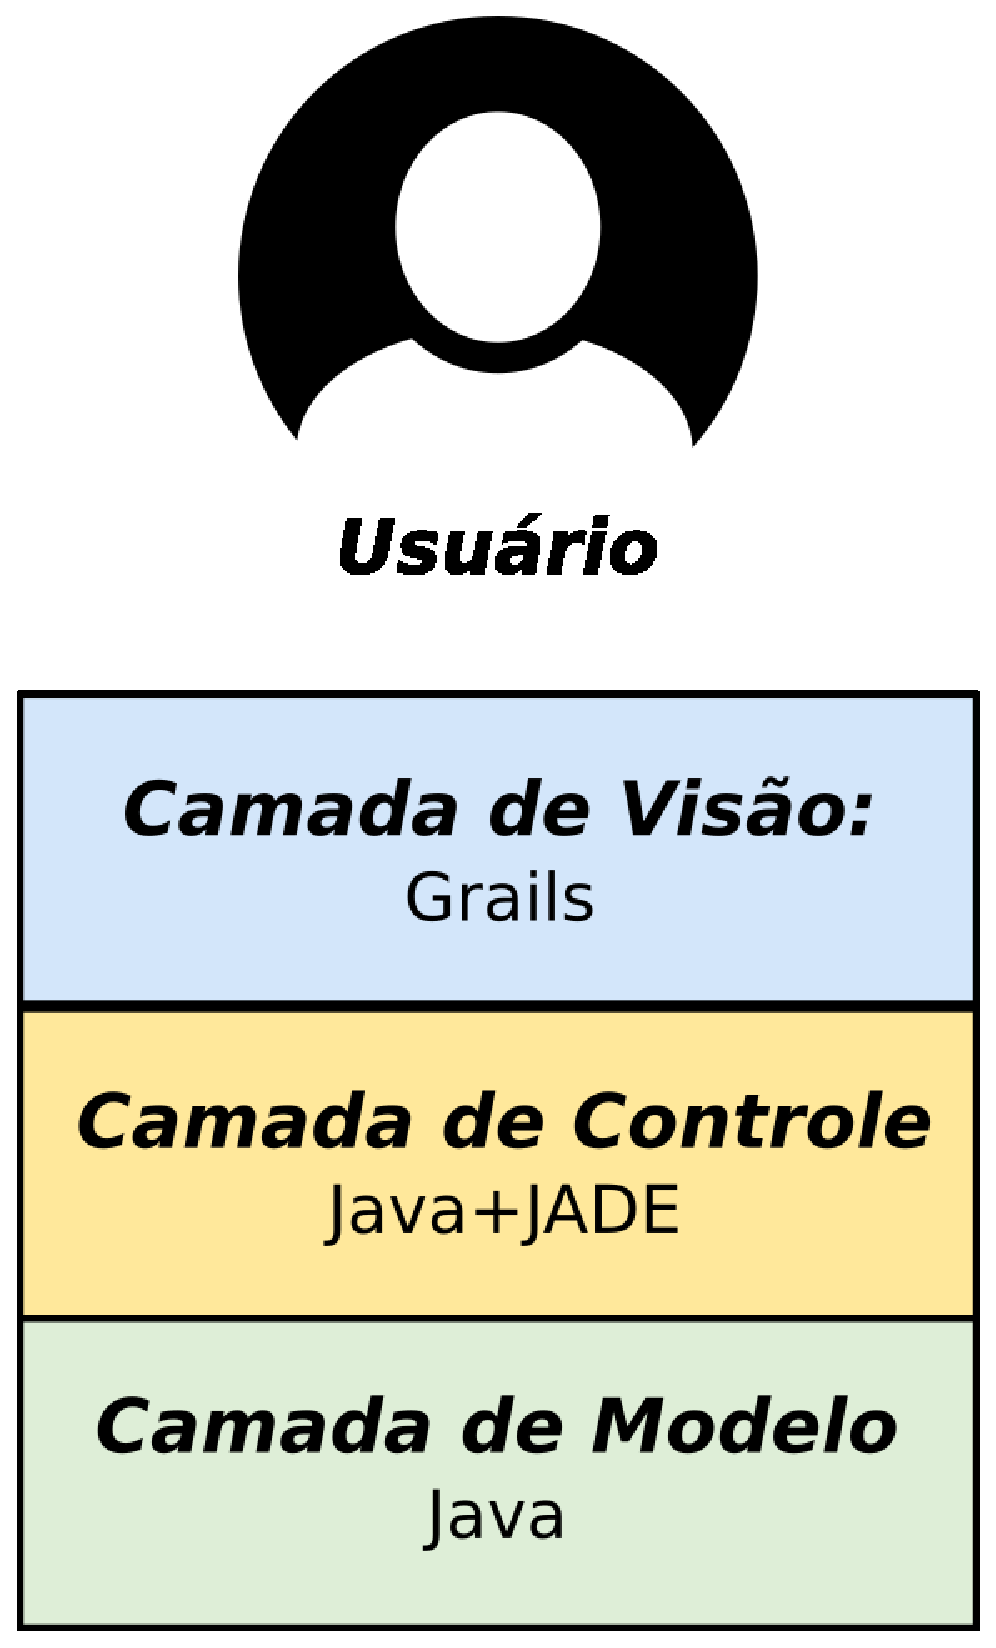
\includegraphics[width=0.6\textwidth]{figuras/arquiteturaVisaoGeral}
\newline{Figura 01:Arquitetura visão Geral}
\end{figure}

A Camada de Controle contém o pacote core. No pacote core estão concentrados os códigos que implementam os agentes comportamentais propostos e suas classes de suporte, concentra-se neste pacote de maneira adicional, uma estrutura proposta para futura refatoração arquitetural da ferramenta, no tocante aos comportamentos dos agente. O tópicos seguintes apresentam mais detalhes dos agentes implementados contidos neste pacote.

A Camada de Modelo contém o pacote suport, este dividido em três subpacotes - financial, util  e statistical. De maneira sucinta,  as classes  contidas no subpacote financial são responsáveis por prover o mecanismo de estratégias financeiras a serem utilizadas pelos agentes comportamentais da Ferramenta de Software. As classes contidas no subpacote statistical são responsáveis por prover mecanismos de calculos estatisticos utilizados por agentes do tipo Caçador (Hunter) para selecionar Ações  compatíveis com os perfis abordados pela Ferramenta, elas são utilizadas ainda pelos agentes do  tipo Gestor (Manager) para realizar o controle de risco envolvido em uma carteira de Ações. As classes contidas no pacote util, são responsáveis por prover o mecanismo de persistência de dados no MongoDB. Vale ressaltar que a comunicação entre as camadas de Visão e Controle é feita via banco de dados, como ilustrado na figura 2.


\begin{figure}[h]
\centering
\label{f2}
\includegraphics[width=0.9\textwidth]{figuras/comunicacao}
\newline{Figura 02: Comunicação entre camadas}
\end{figure}

\subsection{Pacote Core}

O pacote core contém as classes que implementam os Agentes comportamentais utilizados na Ferramenta de Software desenvolvida. Ele contém o subpacote agent e este por sua vez contém  os subpacotes behaviours,  util e suport.   O subpacote util contém classes responsáveis por realizar testes funcionais de comportamentos de agentes, como apresentado no figura 3.   As Classes AgentA e AgentB tem o propósito de realizar  testes de comunicação e comportamentos , esta estratégia foi necessária uma vez que a plataforma JADE até a data de publicação deste documento carecia uma estrutura adequada para testes de comportamentos. As Classes StockAgent, SimulationBehaviour, StocksInMemory e Simulation Setup compõe uma estrutura pensada pelo desenvolvedor para simular a Ferramenta quando não houver conexão com a internet.

O pacote behaviours contém comportamentos isolados a serem agregados a agentes que necessitarem deles. Durante o desenvolvimento da Ferramenta proposta e após seguir as práticas adotadas pelas literaturas relacionadas à implementação de agentes com o JADE, o desenvolvedor elaborou uma arquitetura baseada em interfaces de maneira a reduzir o acoplamento de classes que implementam agentes comportamentais, bem como facilitar futuras manutenções evolutivas e corretivas. Esta arquitetura contém uma interface denominada ProcedureBehaviour e uma classe concreta denominada CommunicationBehaviour, e é uma sugestão de manutenção evolutiva para a Ferramenta de Software, figura 4.

\begin{figure}[h]
\centering
\label{f3}
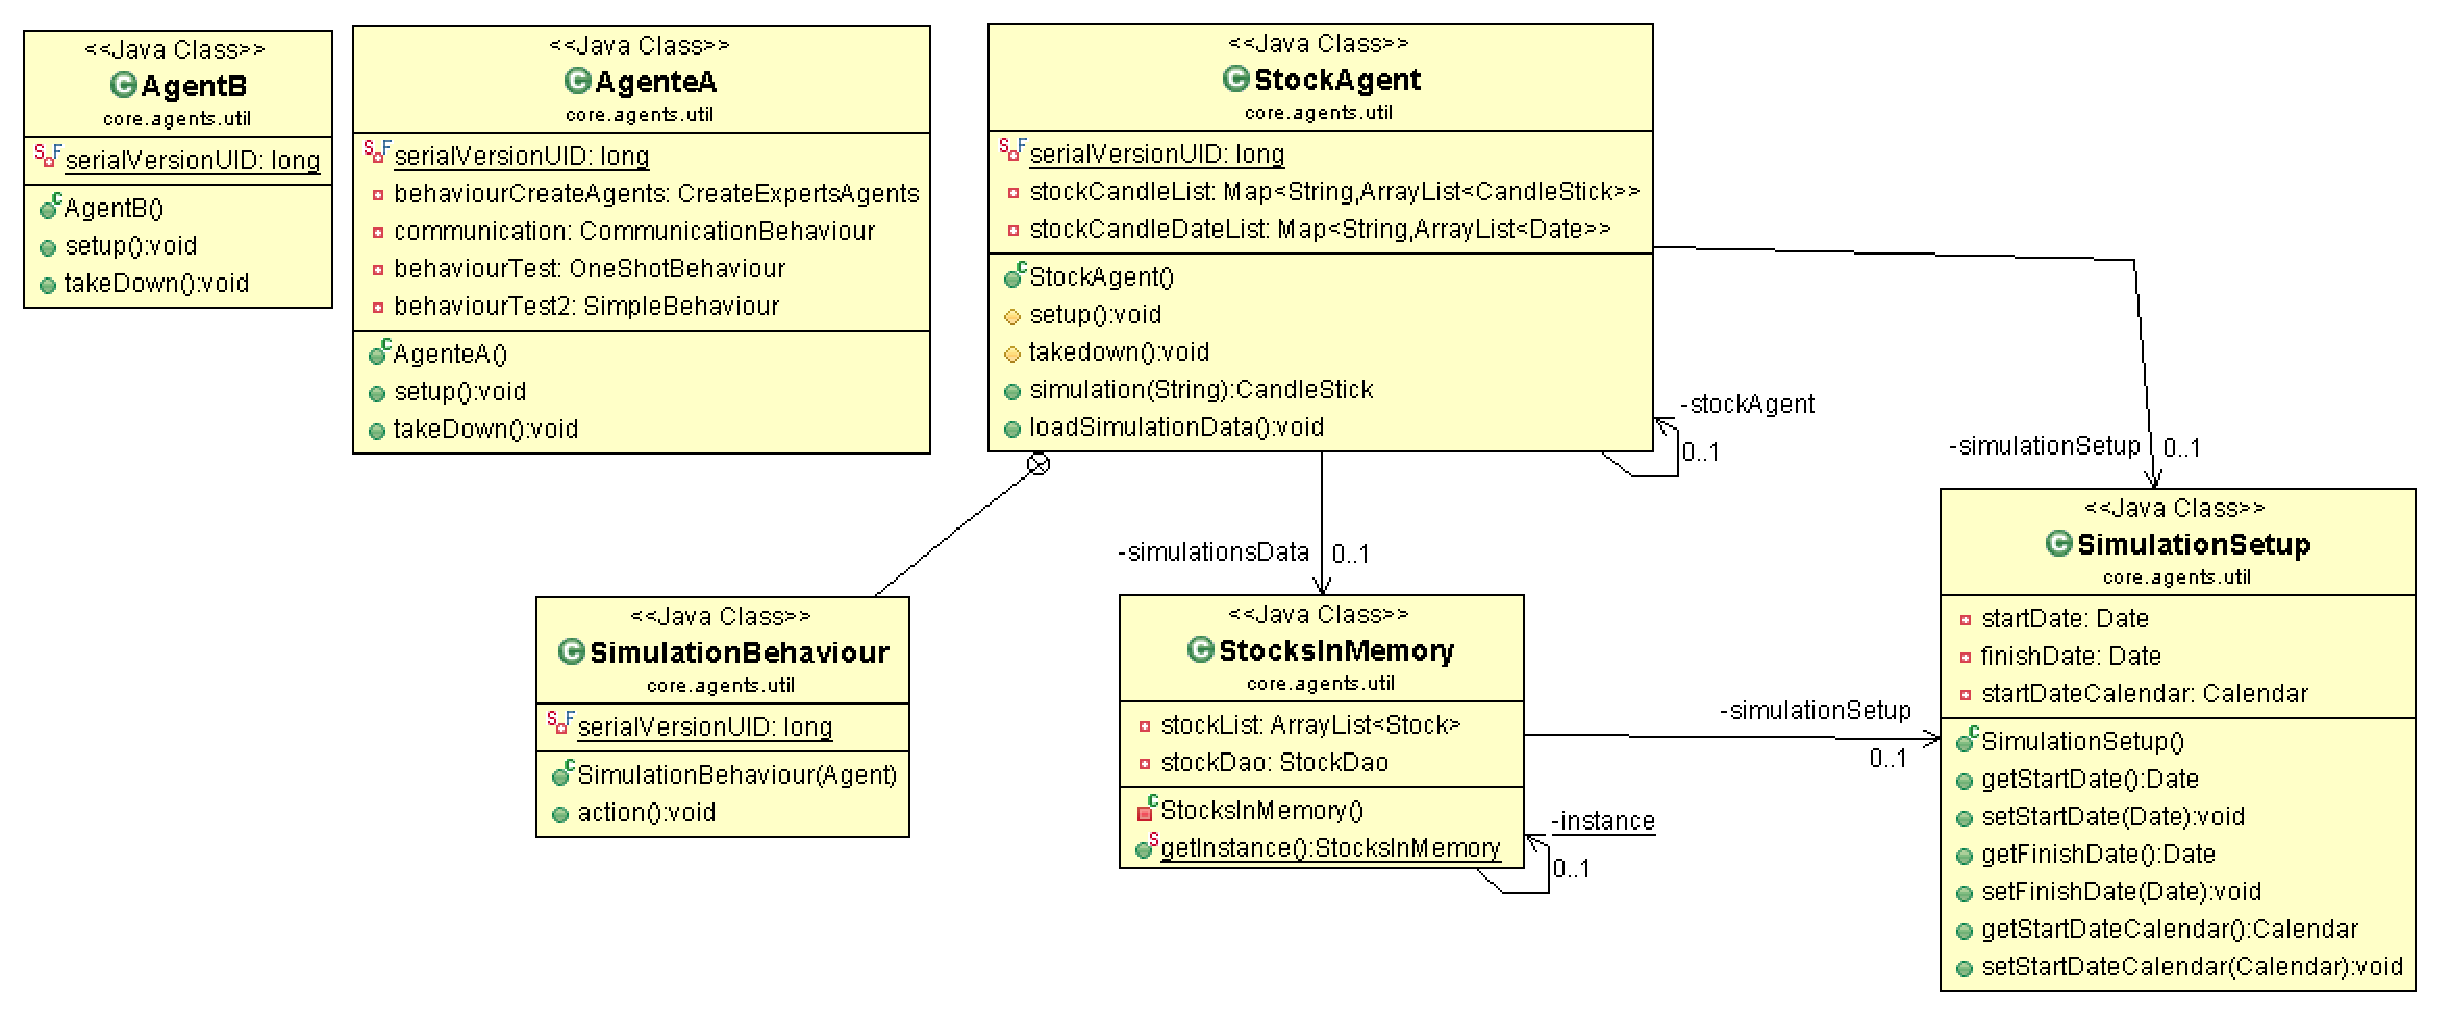
\includegraphics[width=0.9\textwidth]{figuras/pacoteAgents_Util}
\newline{Figura 03: Classes de Apoio}
\end{figure}

A Classe CommunicationBehaviour implementa o comportamento em comum entre os agentes comportamentais que é receber mensagens de outros agentes e responder estas mensagens através da execução de um comportamento. Esta classe dispõe de um mecanismo de adição de comportamentos, na qual para que essa adição seja feita é necessário informar a classe, os atributos ConversationID e uma classe concreta ProcedureBehaviour. Um classe agente comportamental pode utilizar uma classe ProcedureBehaviour sem a necessidade de utilizar a classe CommunicationBehaviour. Esta classe agente pode utilizar da agregação para aplicar o seu conjunto de comportamentos, assim reduzindo o acoplamento da classe e aumentando sua coesão.

\begin{figure}[h]
\centering
\label{f4}
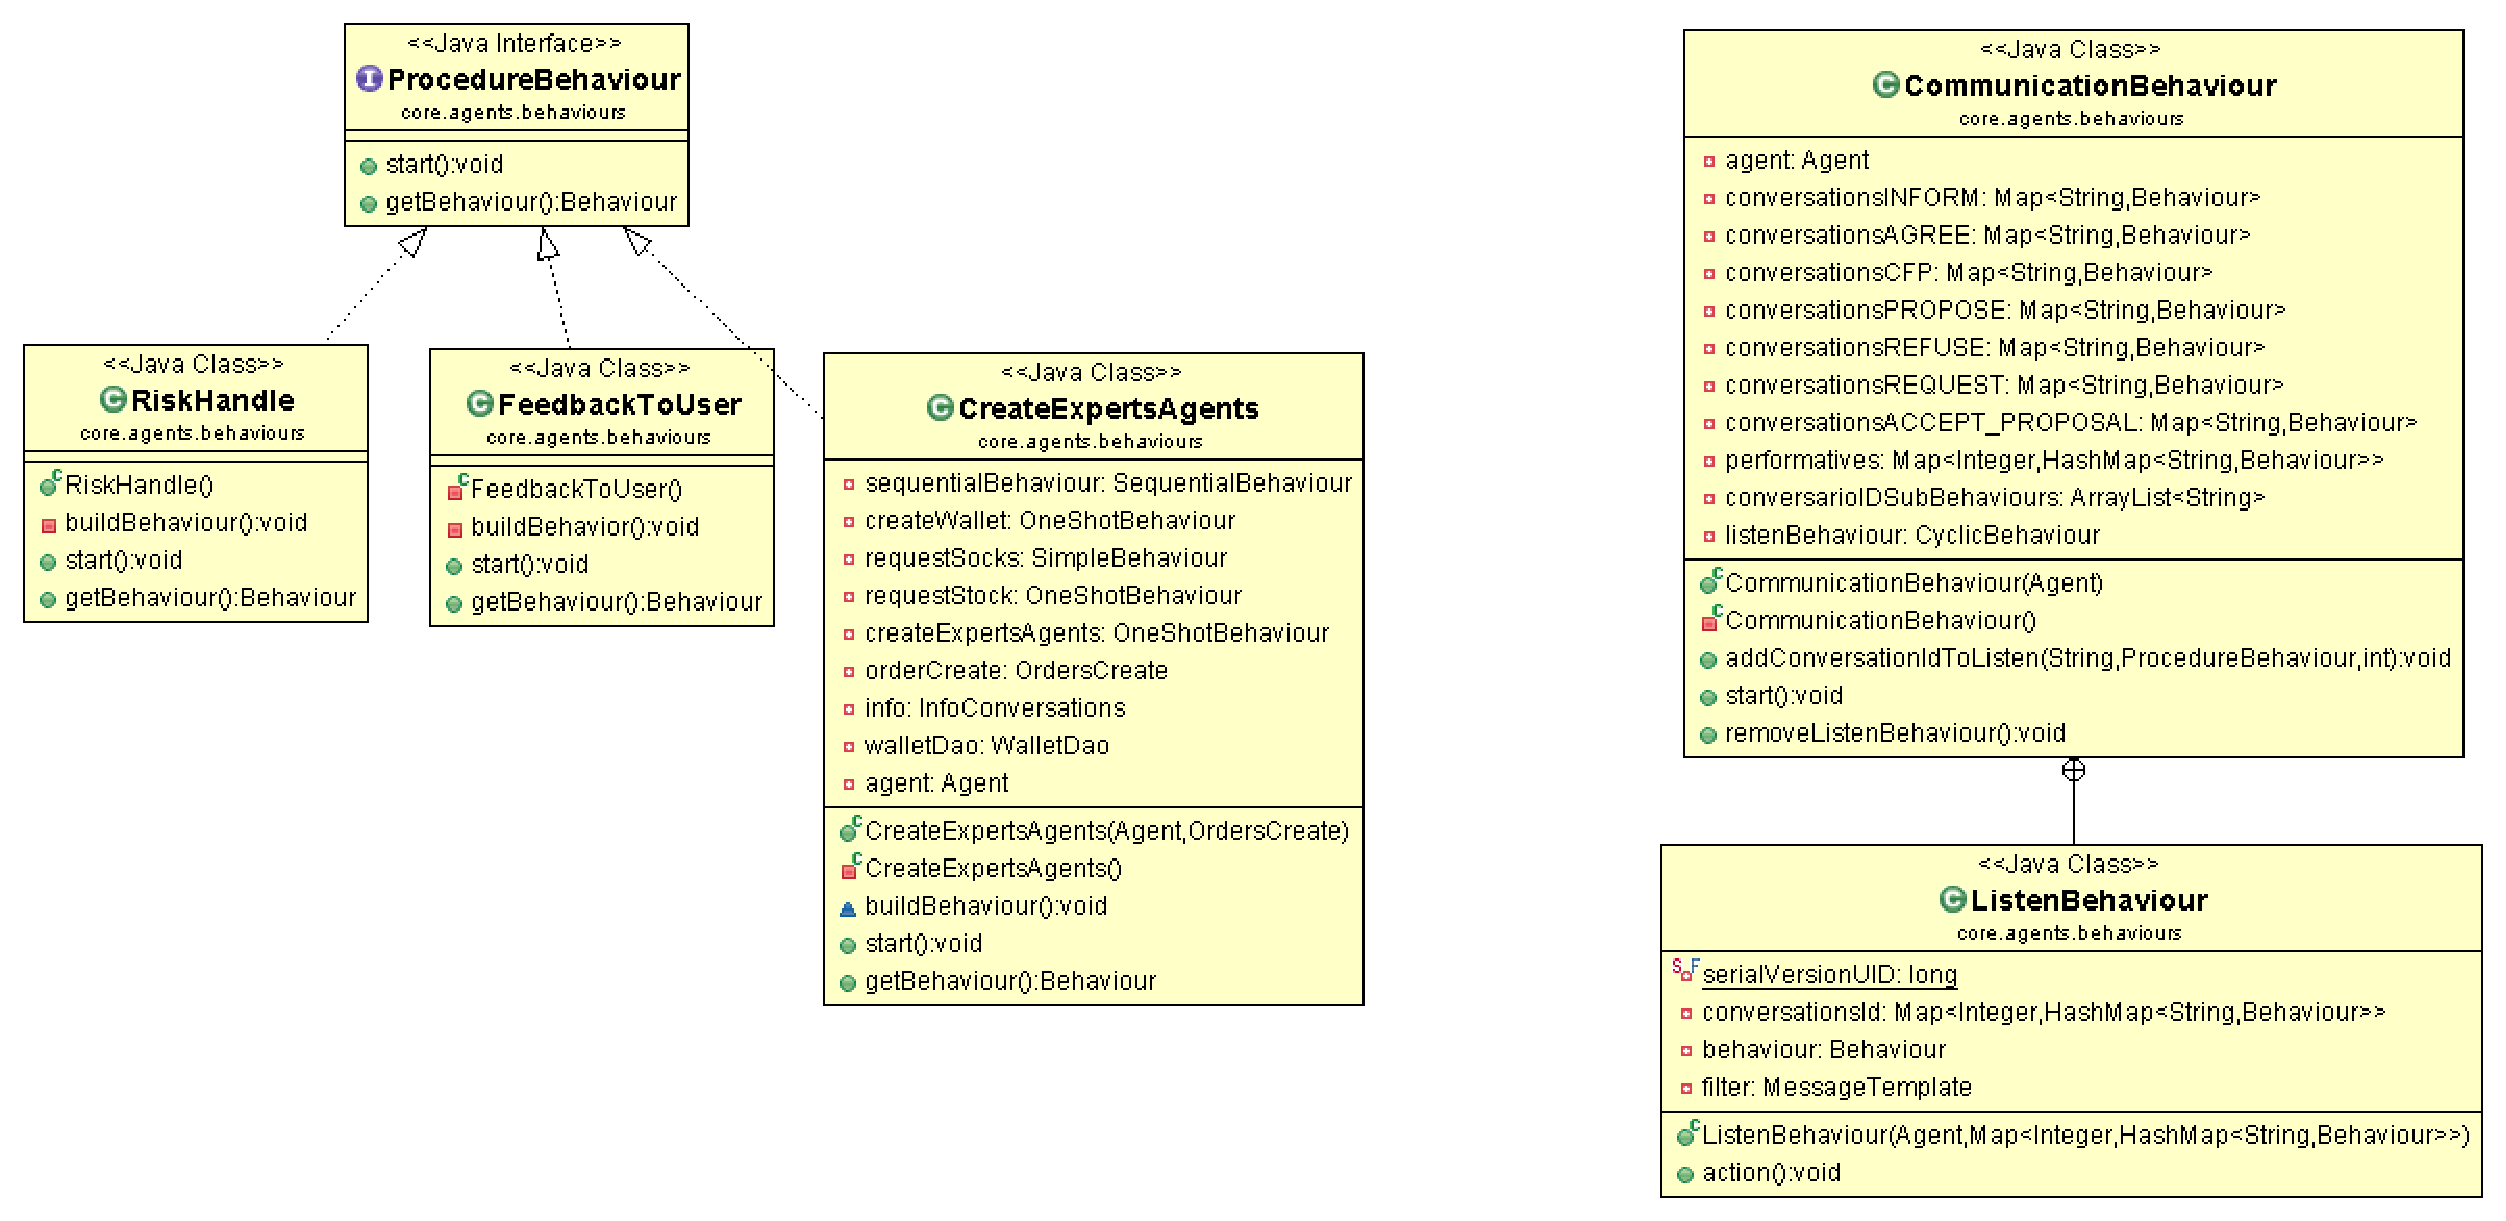
\includegraphics[width=0.9\textwidth]{figuras/pacoteBehaviours}
\newline{Figura 04: Arquitetura sugerida para refatoração arquitetural}
\end{figure}

\subsubsection{Agentes implementados}

Conforme proposto no capítulo 4, Foram implementados os 3 tipos de agentes de Software planejados: (i) Agente Gestor; (ii) Agente Especialista; (iii) Agente Caçador. No entanto, verificou-se a necessidade em criar um quarto tipo de Agente de Software, o Agente Criador. Este responsável por auxiliar na comunicação entre usuários web com seus respectivos Agentes de Software. 

\subsubsubsection{Agente Gestor (Manager)}

O Agente do tipo Gestor é o responsável por administrar a carteira de ações dos usuários, ações que por sua vez são acompanhadas por Agentes Especialistas. Ele autoriza uma compra ou venda de ações analisadas pelos Agentes Especialistas, vale ressaltar que essa autorização passa pelo usuário vinculado ao grupo de Agentes. O Agente Gestor, de maneira autônoma, faz o monitoramento de risco envolvido na carteira de ações administrada. Bem como, executa o processo de montagem de carteira de maneira alinhada com o perfil escolhido pelo usuário. De acordo com as responsabilidades descritas no capitulo 4, foram implementadas as seguintes responsabilidades: 

\begin{itemize}

	\item \textbf{Criar e excluir um ou mais Agentes Especialistas}\newline\newline
	Todo Agente Gestor é criado pelo Agente Criador presente no servidor. A figura 5 ilustra o processo de criação dos Agentes especialistas de acordo com o perfil escolhido pelo usuário. Após criados os Especialistas, é iniciado o processo de montagem de carteira de ações. Apresentado no tópico seguinte.
\begin{figure}[h]
\centering
\label{f5}
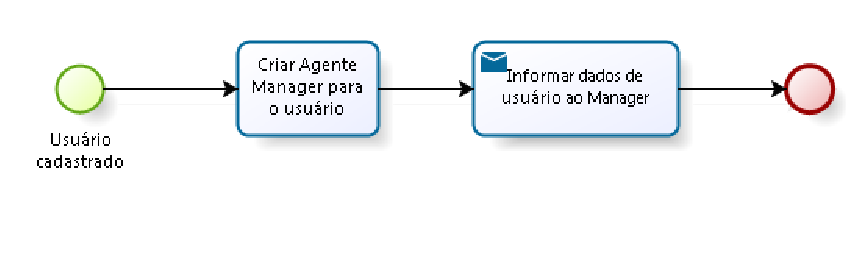
\includegraphics[width=0.9\textwidth]{figuras/f29}
\newline{Figura 5: Processo de criação dos Agentes do tipo Gestor}

\end{figure}

	\item \textbf{Montar carteiras de ações}\newline\newline
	A figura 6 ilustra o processo de montagem de uma carteira de ações, bem como o processo de rateio de ações entre os Agentes Especialistas vinculados ao grupo de Agentes. Vale ressaltar que de acordo com o processo previsto no capítulo 4, as ações escolhidas são alinhadas com o perfil escolhido pelo próprio usuário.  \newline
	
	O processo de montagem de carteira de ações inicia-se no momento em que o um Agente Gestor é instanciado no servidor. Após ser instanciado, o Agente Gestor recebe do Agente criador uma mensagem contendo informações do usuário tais como: (i) Nome; (ii) Valor investido; e (iii) Perfil escolhido. O Agente Gestor envia uma mensagem ao Agente Caçador de Ações solicitando um grupo de ações compatíveis ao perfil escolhido pelo usuário, figura 7. Após escolher as ações, o Agente Gestor faz o rateio entre os Agentes Especialistas. Por fim, ao concluir os processos de montagem de carteira de ação e rateio, o Agente Gestor inicia o processo contínuo de monitoramento do risco na carteira, figura 8.



\begin{figure}[h]
\centering
\label{f6}
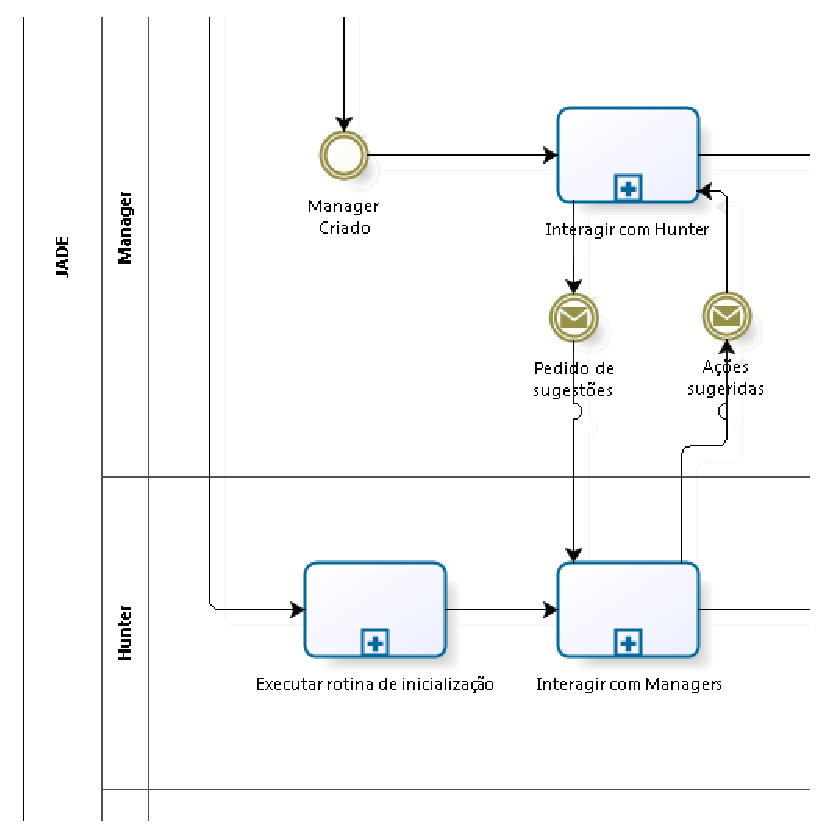
\includegraphics[width=0.7\textwidth]{figuras/f31}
\newline{Figura 6: Processo de montagem de uma Carteira de Ações}
\end{figure}

\begin{figure}[h]
\centering
\label{f7}
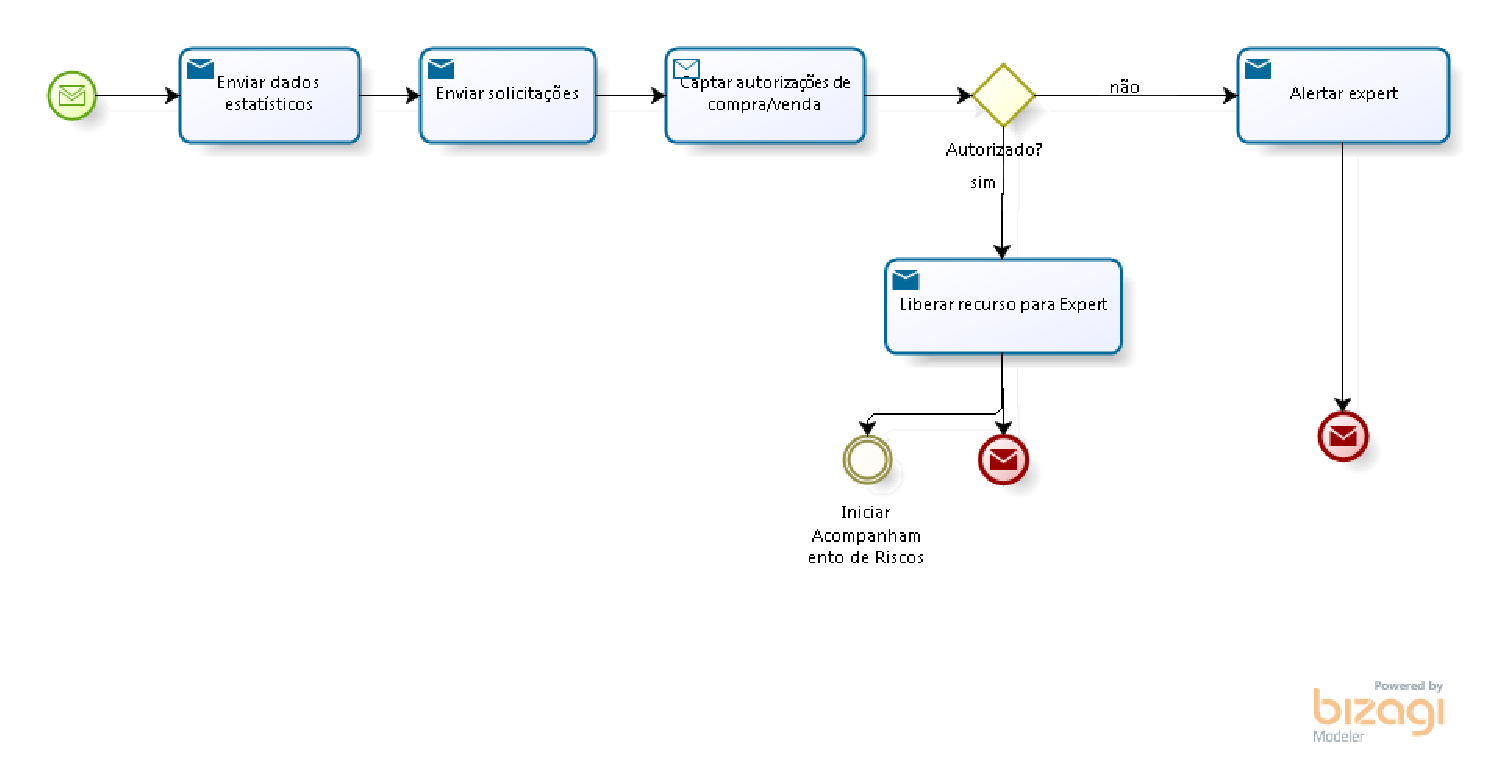
\includegraphics[width=0.9\textwidth]{figuras/f34}
\newline{Figura 7: Processo Troca de Mensagens Agente Gestor e Agente Criador}
\end{figure}


\begin{figure}[h]
\centering
\label{f8}
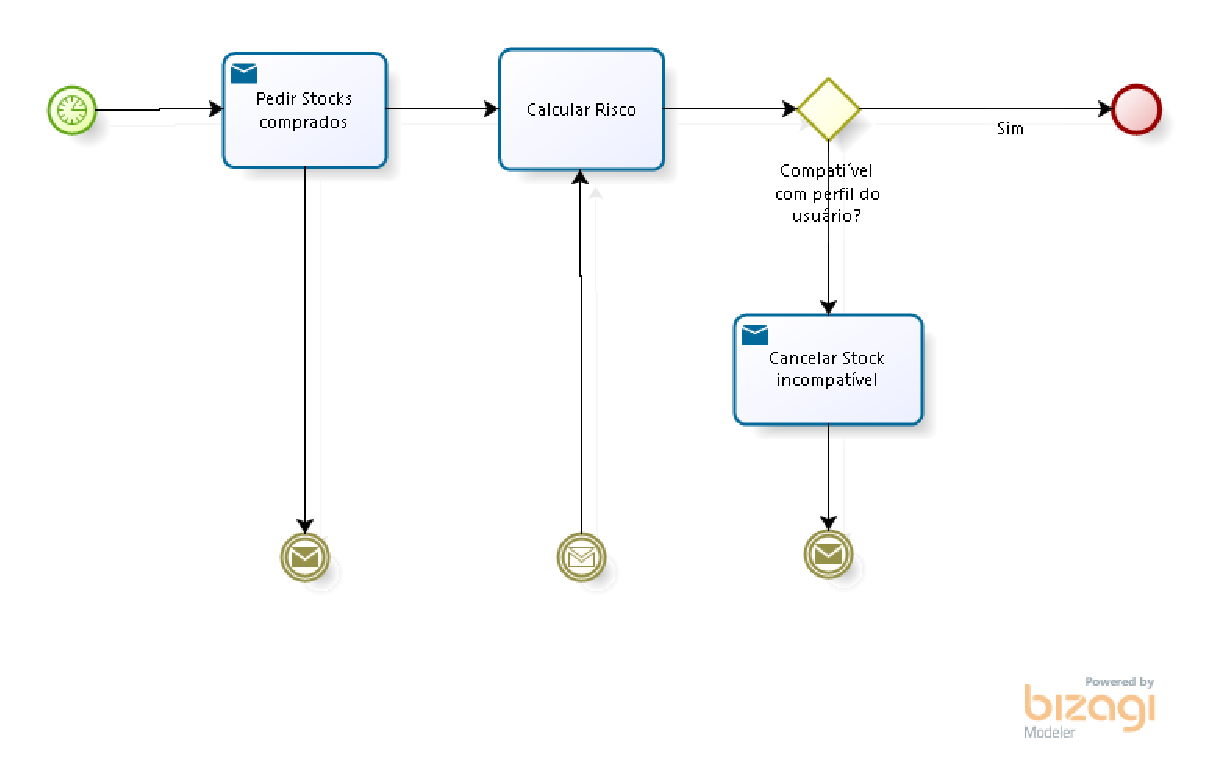
\includegraphics[width=0.9\textwidth]{figuras/f37}
\newline{Figura 8: Monitoramento de risco da carteira de ações}
\end{figure}
\item \textbf{Gerir careiras de ações}\newline\newline
Foi implementado no Agente Gestor um comportamento cíclico responsável por monitorar os riscos envolvidos na carteira de ações, que por sua vez acompanhadas por Agentes Especialistas. O Agente Gestor é capaz de cancelar uma operação de compra, caso esta represente um grau de risco incompatível com o perfil escolhido pelo usuário, figura 9.

\begin{figure}[h]
\centering
\label{f9}
\includegraphics[width=0.9\textwidth]{figuras/f38}
\newline{Figura 9: Acompanhamento de risco em operações}
\end{figure}
\end{itemize}

\subsubsubsection{Agente Especialista (Expert)}

Conforme descrito no capítulo 4, o Agente Especialista é o Agente responsável por realizar leituras constantes do mercado de valores em busca de novas cotações das ações sob sua responsabilidade. Ele é criado pelo seu Agente Gestor e executa estratégias compatíveis com o perfil escolhido pelo usuário, recebe ainda um grupo de ações na qual será responsável. Durante o Desenvolvimento, verificou-se necessário transferir a responsabilidade de mensurar risco de estratégias para o seu Agente Gestor, e após implementação verificou-se empiricamente que executar uma rotina de simulação poderia onerar o servidor devido ao consumo de memória ao manipular objetos Candlesticks em grande quantidade. Com isso, foram implementadas as seguintes responsabilidades: (i) Aplicar estratégias que ofereçam o maior lucro possível compatível com o perfil escolhido pelo usuário; e (ii) Solicitar autorização para realizar compra ou venda de ações, figura 11.


\begin{figure}[h]
\centering
\label{f10}
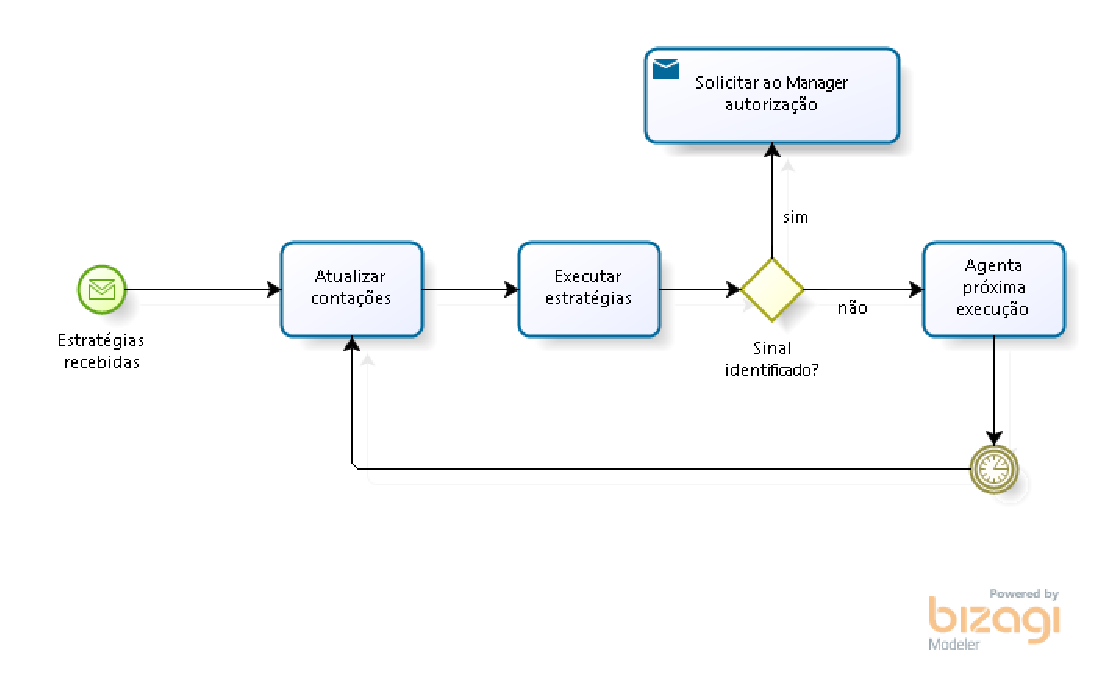
\includegraphics[width=0.9\textwidth]{figuras/f40}
\newline{Figura 10: Acompanhamento de risco em operações}
\end{figure}

\subsubsubsection{Agente Caçador (Hunter)}
Conforme descrito no capitulo 4, o Agente Caçador é responsável por fazer buscas constantes de cotações de ações presentes na bolsa de valores e trabalhadas pela ferramenta e realizará uma categorização destas ações através de valores estatísticos, tais como: (i) retorno médio diário; (ii) retorno médio 15 e 30 dias; (iii) variância média diária; e (iv) variância média 15 e 30 dias. Através destes valores, o Agente Caçador seleciona grupos de ações compatíveis com os perfis informados por Agentes Gestores no procedimento de montagem de carteira. De acordo com as responsabilidades descritas no capitulo 4, foram implementadas as seguintes responsabilidades: (i) Busca e Seleção das melhores ações a se investir, estas ações variam de acordo com o perfil de usuário tratado pelos Agentes Gestores. O processo é ilustrado na figuras 11; e (ii) categorização de ações através de valores estatísticos, o Agente caçador faz cálculos estatísticos frequentes dada ação abordada na ferramenta e os utiliza como parâmetro de escolha para selecionar ações para atender as solicitações dos Agentes Gestores, como ilustrado na figuras 12.

\begin{figure}[h]
\centering
\label{f11}
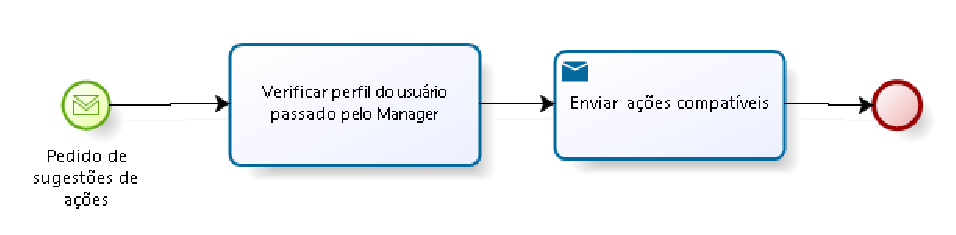
\includegraphics[width=0.9\textwidth]{figuras/f42}
\newline{Figura 11: Processo de escolha de ações}
\end{figure}

\begin{figure}[h]
\centering
\label{f12}
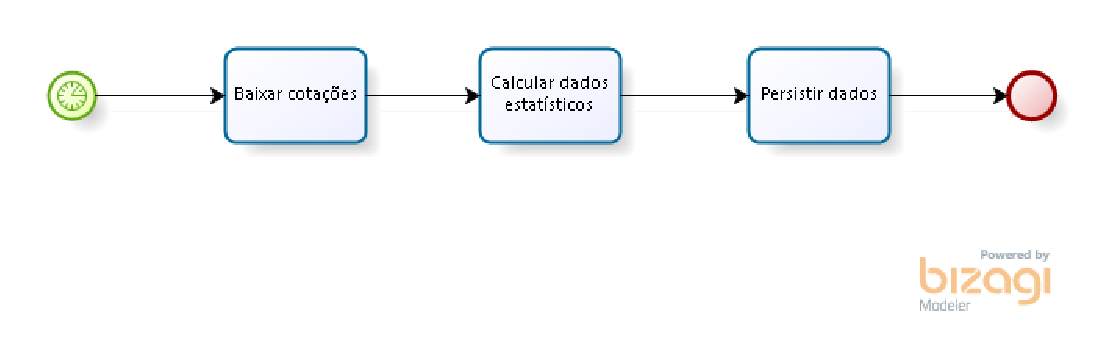
\includegraphics[width=0.9\textwidth]{figuras/f44}
\newline{Figura 12: Persistência de valores estatísticos por ação}
\end{figure}

\subsubsubsection{Agente Criador (Criator)}

Este agente não foi previsto no capitulo 4, porém durante a implementação verificou-se a necessário criar um tipo de Agente para auxiliar na comunicação entre os usuários e seus respectivos grupos de Agentes. Assim como o Agente Caçador, existe apenas um agente Criador para cada servidor. Suas responsabilidades são: (i) Monitorar a criação de novas contas. O usuário quando cria uma conta o Agente Criador captura as informações repassadas pelo usuário, cria um Agente Gestor para este usuário e o informa através de uma mensagem com informações do usuário tais como nome, valor investido e perfil escolhido; (ii) Monitorar \textit{Log In} de usuários.  Quando um usuário autentica-se na ferramenta, o Agente Criador informa ao seu Agente Gestor para que o mesmo comunique-se com seu usuário, a comunicação entre o Agente Gestor e seu respectivo usuário é demonstrado na figura 15, bem como todas funcionalidades apresentadas neste documento.

\subsection{Pacote Suport}

Este pacote comporta as classes de suporte ao funcionamento da Ferramenta de Software desenvolvida, nele estão classes relacionadas a persistência de dados e a estratégias financeiras utilizadas pelos agentes comportamentais desenvolvidos. A figura 13 ilustra de maneira geral a composição do pacote suport. 

\begin{figure}[h]
\centering
\label{f13}
\includegraphics[width=0.9\textwidth]{figuras/pacoteSuport}
\newline{Figura 13: Pacote Suport}
\end{figure}

O pacote suport é divido em três importantes subpacotes, financial, util e statistical. No pacote financial estão concentradas as classes responsáveis por prover as estratégias financeiras utilizadas pelos agentes Especialistas. O subpacote statistical contém classes que dispõe de cálculos estatísticos utilizados pelo agente Caçador para encontrar Ações compatíveis com os três perfis de usuários abordados pela ferramenta. O subpacote util contém as classes responsáveis pela persistência de dados bem como requisições http de novas cotações.

O pacote suport é essencial para futuras manutenções evolutivas da ferramenta, pois para adicionar novas estratégias basta criar novas classes com estas estratégias e implementar a interface Strategy. A figura 14 apresenta o diagrama das duas principais estratégias abordadas na Ferramenta de Software. Caso a manutenção evolutiva tenha como objetivo abordar outras Bolsa de Valores ou mesmo consumir dados diretamente da BM\&FBovespa, o pacote candidato a manutenção será o requests. Pois este, contém as classes que implementam a obtenção de dados e a lógica de armazenamento destes dados.

\begin{figure}[h]
\centering
\label{f14}
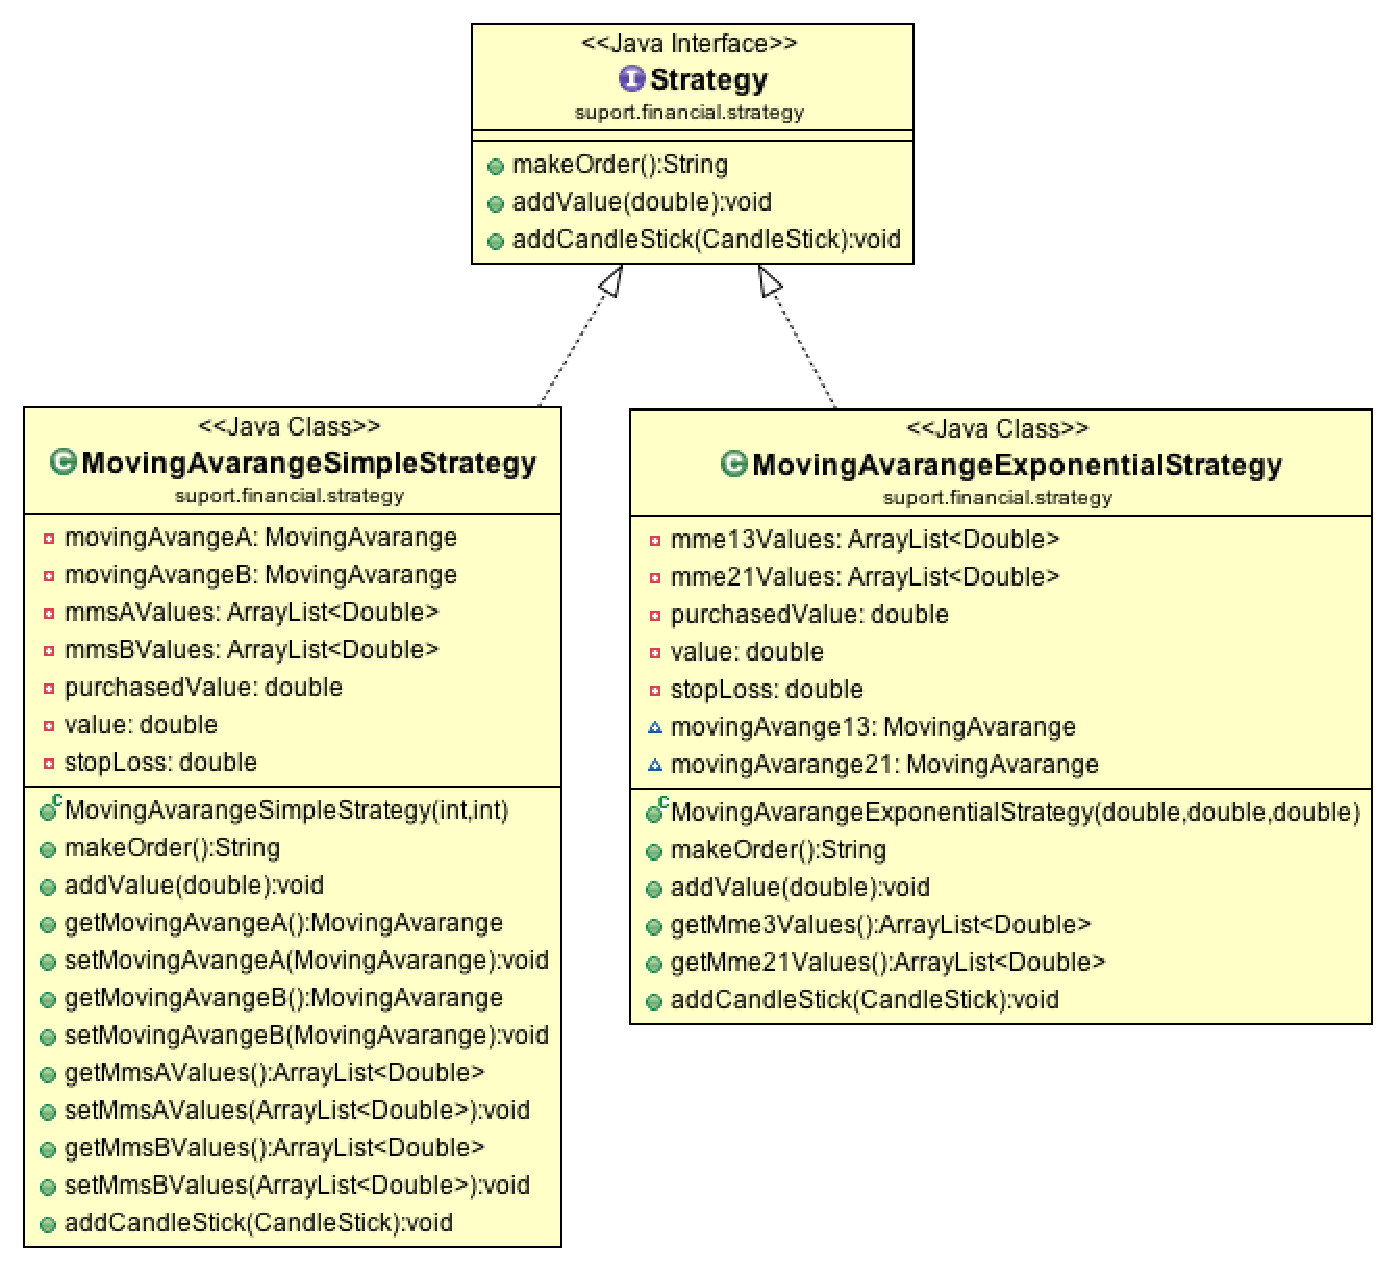
\includegraphics[width=0.9\textwidth]{figuras/estrategiasClasses}
\newline{Figura 14: Estratégias Financeiras}
\end{figure}

\begin{figure}[h]
\centering
\label{f15}
\includegraphics[width=0.9\textwidth]{figuras/f46}
\newline{Figura 15: Visão geral da Ferramenta}
\end{figure}

\section{Ferramentas}



\begin{center}
\begin{longtable}{| p{4cm} | p{4cm} |p{4cm}|}
\caption*{Ferramentas adotadas} \\
\hline
\textbf{Nome} & \textbf{Versão} & \textbf{Responsabilidade} \\ \hline
\endfirsthead
\multicolumn{2}{c}%
{\tablename\ \thetable\ -- \textit{Continuação da página anterior}} \\
\hline
\textbf{Nome} & \textbf{Versão} & \textbf{Responsabilidade}\\ \hline
\endhead
\hline \multicolumn{2}{c}{\textit{Continuaçao na próxima página}} \\
\endfoot
\hline
\endlastfoot

	JADE	&14.3.2	&Prover Agentes Comportamentais\\ \hline
	Grails	&2.4.3	&Prover Interface com usuários\\ \hline
	MongoDB	&3.0.2	&Banco de Dados Não Relacional\\ \hline
	Maven	&3.3.3	&Gerencia de dependências\\ \hline
	Java JDK	&1.7.0\_79	&Copilador\\ \hline
	Eclipse Luna	&4.4.0	&IDE

	

\label{t1}
\end{longtable}
\end{center}



\end{apendicesenv}
